\documentclass[12pt, a4paper]{memoir} % for a short document
\usepackage[french,english]{babel}

\usepackage [vscale=0.76,includehead]{geometry}                % See geometry.pdf to learn the layout options. There are lots.
%\geometry{a4paper}                   % ... or a4paper or a5paper or ...
%\geometry{landscape}                % Activate for for rotated page geometry
%\OnehalfSpacing
% \setSingleSpace{1.05}
%\usepackage[parfill]{parskip}    % Activate to begin paragraphs with an empty line rather than an indent


%===================================== packages
\usepackage{lipsum}
\usepackage{graphicx}
\usepackage{amsmath}
\usepackage{amssymb}
\usepackage{amsthm}
\newtheorem{theorem}{Theorem}[chapter]
\newtheorem{proposition}[theorem]{Proposition}
\newtheorem{corollary}[theorem]{Corollary}
\newtheorem{lemma}[theorem]{Lemma}
\theoremstyle{definition}
\newtheorem{definition}[theorem]{Definition}
\usepackage{fullpage}
\usepackage{mathptmx} % font = times
\usepackage{helvet} % font sf = helvetica
\usepackage[latin1]{inputenc}
\usepackage{relsize}
\usepackage[T1]{fontenc}
\usepackage{tikz}
\usepackage{booktabs}
\usepackage{textcomp}%textquotesingle
\usepackage{multirow}
\usepackage{pgfplots}
\pgfplotsset{compat=1.17}
\usepackage{url}
\usepackage{xurl}
\usepackage{footnote}
\usepackage{algorithm}
\usepackage{algpseudocode}
\usepackage{listings}
\usepackage{xcolor}
\usepackage{hyperref}
%============================================
\usetikzlibrary{arrows,arrows.meta,shapes,shapes.geometric,positioning,shadows,trees,fit,backgrounds}
\makesavenoteenv{tabular}
\makesavenoteenv{table}
%==============================================
\def\checkmark{\tikz\fill[scale=0.4](0,.35) -- (.25,0) -- (1,.7) -- (.25,.15) -- cycle;}

\lstdefinestyle{prompt}{
  basicstyle=\ttfamily\footnotesize,
  breaklines=true,
  frame=single,
  columns=fullflexible,
  backgroundcolor=\color{gray!8},
  showstringspaces=false
}
\lstdefinestyle{pyc}{
  basicstyle=\ttfamily\small,
  breaklines=true,
  frame=single,
  columns=fullflexible,
  backgroundcolor=\color{blue!4},
  showstringspaces=false,
  keywordstyle=\color{blue!60!black}\bfseries,
  commentstyle=\color{gray}\itshape
}

%Style des t\^etes de section, headings, chapitre
\headstyles{komalike}
\nouppercaseheads
\chapterstyle{dash}
\makeevenhead{headings}{\sffamily\thepage}{}{\sffamily\leftmark}
\makeoddhead{headings}{\sffamily\rightmark}{}{\sffamily\thepage}
\makeoddfoot{plain}{}{}{} % Pages chapitre.
\makeheadrule{headings}{\textwidth}{\normalrulethickness}
%\renewcommand{\leftmark}{\thechapter ---}
\renewcommand{\chaptername}{\relax}
\renewcommand{\chaptitlefont}{ \sffamily\bfseries \LARGE}
\renewcommand{\chapnumfont}{ \sffamily\bfseries \LARGE}
\setsecnumdepth{subsection}


% Title page formatting -- do not change!
\pretitle{\HUGE\sffamily \bfseries\begin{center}}
\posttitle{\end{center}}
\preauthor{\LARGE  \sffamily \bfseries\begin{center}}
\postauthor{\par\end{center}}
\newcommand{\jury}[1]{%
\gdef\juryB{#1}}
\newcommand{\juryB}{}
\newcommand{\session}[1]{%
\gdef\sessionB{#1}}
\newcommand{\sessionB}{}
\newcommand{\option}[1]{%
\gdef\optionB{#1}}
\newcommand{\optionB} {}

\renewcommand{\maketitlehookd}{%
\vfill{}  \large\par\noindent
\begin{center}\juryB \bigskip\sessionB\end{center}
\vspace{-1.5cm}}
\renewcommand{\maketitlehooka}{%
% NOTE: the original template places university/school crests here via
% 
\includegraphics{pics/logo-uga.png} and 
\includegraphics{pics/logoINP.png}.
% Those image files are institution-owned trademarks and are intentionally
% NOT reproduced in this generated draft; replace the line below with the
% two \includegraphics calls (see comment) once you drop your own copies of
% the crests into pics/.
\vspace{-1.5cm}\noindent{\large\sffamily Universit\'e Grenoble Alpes \hfill Grenoble INP -- Ensimag}\\
% 
\includegraphics[height=12ex]{pics/logo-uga.png}\hfill\raisebox{2ex}{
\includegraphics[height=14ex]{pics/logoINP.png}}\\
\bigskip
\begin{center} \large
Master of Science in Informatics at Grenoble \\
Master Informatique \\
Specialization \optionB  \end{center}\vfill}
% =======================End of title page formatting

\option{Data Science / Databases and Artificial Intelligence}
\title{Cascaded Structured--Semantic Query Processing over Heterogeneous Data\\\vspace{-1ex}\rule{18ex}{0.5pt}\\From SUQL and Batched Semantic Joins to Bayesian-Calibrated Two-Level Cascades}
\author{Anna}
\date{2026} % Delete this line to display the current date
\jury{
Research and engineering project performed at the intersection of database systems and large language models (LLMs), MoSIG / Ensimag, Universit\'e Grenoble Alpes \\\medskip
Under the supervision of:\\
{\itshape (Supervisor name -- to be completed)} \\\medskip
Defended before a jury composed of:\\
{\itshape (Head of the jury -- to be completed)}\\
{\itshape (Jury member 1 -- to be completed)}\\
{\itshape (Jury member 2 -- to be completed)}\\
}
\session{July \hfill 2026}
\setcounter{tocdepth}{4}
\setcounter{secnumdepth}{4}

\newcommand{\answerfn}{\texttt{answer()}}
\newcommand{\eg}{e.g.\ }
\newcommand{\ie}{i.e.\ }

%%% BEGIN DOCUMENT
\begin{document}
\sloppy
\selectlanguage{English} % french si rapport en fran\c{c}ais
\frontmatter
\begin{titlingpage}
\maketitle
\end{titlingpage}

%\small
\setlength{\parskip}{-1pt plus 1pt}

\renewcommand{\abstracttextfont}{\normalfont}
\abstractintoc
\begin{abstract}
Answering natural-language questions that mix structured predicates (e.g.\ release year, film duration, genre) with unstructured predicates over free text (e.g.\ ``the reviews are strongly negative'') requires a query engine that can call a large language model (LLM) as a relational operator. Two execution strategies are commonly used: a \emph{predicate-pushdown} strategy that pushes structured filters into SQL and evaluates the semantic predicate with one LLM call per candidate row (the SUQL-style), and a \emph{batched-join} strategy that packs many rows into a single LLM call and asks the model to execute the whole predicate over a chunk of serialized rows at once (the Trummer-style batch join). We show empirically, on ten held-out, genre-diverse questions against a controlled, auditable $100$-movie pool per question (drawn from a $\sim$25k-row IMDb corpus with paired structured metadata and free-text reviews, each question run ten times per method), that the row-wise strategy is accurate but slow ($117.1$ calls and $115.6$s per question) while the batched strategy is faster ($96.9$ calls, $71.3$s) but visibly less accurate (F1 $0.444$ vs.\ $0.678$). We then utilize a \emph{two-level cascade} to introduce a fast, yet quality preserving pipeline that adds a structured SUQL-style filtering before the Trummer-style batch join block and finally a cheap, uncertainty-aware pre-filter in front of either strategy: rows (or batches) for which the cheap stage is confident are resolved immediately, and only the ones that fall inside a Bayesian-calibrated ambiguity interval are escalated to the expensive stage. Cascading the row-wise strategy (SUQL~V1) improves F1 by $2.7\%$ over the row-wise baseline using about $40\%$ fewer calls. Cascading the batched strategy (Trummer~V1) is the best overall design point: it reaches F1 $0.757$ ($+8.8\%$ over SUQL~V1, $+70.4\%$ over the batched baseline) and the best precision of all four variants ($+14.2\%$ over the row-wise cascade), while using only $1/26$ of the wall-clock time and $1/7$ of the LLM calls of the row-wise cascade, at the cost of a small ($\approx 7\%$) recall regression relative to it. We give the full architecture, pseudocode, prompts, and a Beta-posterior formalization of the calibrated cascade threshold that explains this cost--quality curve.
\end{abstract}
\abstractintoc

\renewcommand\abstractname{Acknowledgement}
\begin{abstract}
I would like to express my sincere gratitude to my supervisor and to the
members of the jury for their invaluable comments and guidance throughout
this project.
\end{abstract}


\renewcommand\abstractname{R\'esum\'e}
\begin{abstract} \selectlanguage{French}
Les questions en langage naturel pos\'ees sur des ensembles de donn\'ees
h\'et\'erog\`enes m\'elangeant colonnes structur\'ees (ann\'ee de sortie,
genre, note) et champs textuels libres (critiques) ne peuvent \^etre
r\'esolues ni par le seul SQL, ni par un grand mod\`ele de langage (LLM)
seul \`a un co\^ut raisonnable. Ce rapport con\c{c}oit, impl\'emente et
\'evalue une famille de moteurs d'ex\'ecution de requ\^etes
structur\'ees--non structur\'ees (dans l'esprit de SUQL) sur un jeu de
donn\'ees IMDb d'environ 25~000 lignes, et \'etudie le compromis entre deux
strat\'egies d'ex\'ecution~: le \emph{predicate pushdown} ligne par ligne
(SUQL) et la \emph{jointure s\'emantique group\'ee} (style Trummer). Nous
introduisons une \emph{cascade \`a deux niveaux}, calibr\'ee par une borne
cr\'edible bay\'esienne (loi B\^eta) sur les log-odds \`a la mani\`ere de
Stretto, qui am\'eliore simultan\'ement le co\^ut et la qualit\'e par
rapport aux deux r\'ef\'erences.
\end{abstract}
\selectlanguage{English}

\cleardoublepage

\tableofcontents* % the asterisk means that the table of contents itself isn't put into the ToC
\normalsize

\mainmatter
\SingleSpace
%==============================CHAPTERS==================
\chapter{Introduction}
\label{chap:intro}

\section{Motivation}

Modern data pools are rarely purely relational. A movie catalogue such as
IMDb, for instance, pairs a structured relation -- title, release year,
genre, average rating, cast -- with a large body of free-text evidence:
plot summaries and, above all, user reviews. A realistic information need
over such a pool routinely mixes both modalities in a single question:

\begin{quote}
\emph{``Which movies released in 1998 have reviews expressing an overall
negative, critical, or strongly unfavorable opinion of the movie?''}
\end{quote}

The first half of this question -- \texttt{year = 1998} -- is a textbook
relational predicate: it is answered exactly, cheaply, and instantly by a
\texttt{WHERE} clause against an indexed column. The second half --
\emph{``expressing an overall negative, critical, or strongly unfavorable
opinion''} -- is a semantic predicate over unstructured text that no
amount of indexing or exact-match SQL can express. It requires either a
learned text classifier or, at the level of accuracy and flexibility we
target here, a large language model (LLM) invoked as a query operator.

The engineering problem this report addresses is therefore not ``can an
LLM answer this question'' -- it clearly can, given enough context and
enough calls -- but rather: \emph{how do we build a query engine that
answers such questions correctly, while keeping the number of LLM calls
and the wall-clock latency as low as possible?} This is a cost-vs-quality
optimization problem with the same flavor as classical query optimization
(operator ordering, selectivity estimation, pushdown), except that one of
the ``operators'' is a probabilistic, expensive, non-relational function:
the LLM.

\section{Problem Statement}
\label{sec:intro-problem}

Formally, we are given:
\begin{itemize}
  \item a structured relation $R$ with schema
        $(\mathit{id}, \mathit{year}, \mathit{genre}, \mathit{rating},
        \mathit{cast}, \dots)$, $|R| \approx 25{,}000$ rows;
  \item a free-text relation $D(\mathit{id}, \mathit{review})$, in a
        one-to-one (or one-to-few) correspondence with $R$ on
        $\mathit{id}$;
  \item a natural-language query $Q$ that decomposes (possibly only
        implicitly) into a structured predicate $\sigma_S$ over $R$'s
        columns and a semantic predicate $\sigma_U$ over $D$'s text,
        joined conjunctively: $Q \equiv \sigma_S \wedge \sigma_U$.
\end{itemize}
The desired output is the JSON-serializable result set
$\{\, r \in R \bowtie D : \sigma_S(r) \wedge \sigma_U(r) \,\}$, and the
desired \emph{system} property is that it produce this set (i) as close
as possible to a hand-verified gold answer set (measured by precision,
recall, F1), (ii) with as few LLM calls as possible, and (iii) with as
low wall-clock latency as possible. These three objectives are in
tension, and the remainder of this report is an account of how far a
principled combination of classical query-optimization ideas (predicate
pushdown, operator reordering, selectivity-aware short-circuiting) and
modern LLM-serving ideas (batched invocation, confidence calibration,
cascaded inference) can push the achievable trade-off surface.

All code, prompts, and benchmark data referenced in this report are
drawn from the project repository at
\url{https://github.com/AnnaRemi/ENSIMAG-AI-M2-final-project}, branch
\texttt{agent/consolidate-four-method-benchmarks}. Experiments
(Chapter~\ref{chap:experiments}) are run against controlled,
$100$-row-per-question subdatasets drawn from the $\sim$25{,}000-row
canonical corpus above, rather than against the full corpus directly,
so that every question has a known, auditable gold set of a fixed size
(Section~\ref{sec:10q-suite}).

\section{What Existed Before This Project}

Two execution strategies were already implemented and benchmarked before
the work reported here, and both are treated as \emph{baselines} rather
than as strawmen: they are each the right choice for some regime of the
problem, and understanding exactly why is what motivates the cascaded
design of Chapter~\ref{chap:cascading}.

\begin{description}
\item[\textbf{SUQL baseline.}] Following the design of SUQL~\cite{suql},
  the structured predicate $\sigma_S$ is compiled to SQL and evaluated
  first, and the semantic predicate $\sigma_U$ is evaluated by issuing
  one \answerfn{} call per surviving row to an LLM. Quality is high
  because every row is judged individually and in full context, but the
  number of LLM calls equals $|R_{\sigma_S}|$ -- the size of the
  structurally filtered relation -- so the strategy does not scale
  gracefully when the structured predicate is not very selective.
\item[\textbf{Trummer baseline.}] The structured relation and the review
  relation are kept as two \emph{separate} collections -- deliberately,
  by design, with \emph{no} SUQL-style structured pushdown -- and the
  LLM itself is asked to join a block of one collection against a block
  of the other while simultaneously applying the semantic predicate, an
  adaptive block-pair join over the \emph{entire} candidate pool. This
  is far cheaper in calls and wall time than row-wise judgment, but is
  measurably less accurate: the model must recover row identity from
  block text and perform the join itself, and errors (id drift,
  incomplete coverage of a block's decisions) compound without any
  structural narrowing of the pool it has to cover.
\end{description}

Both baselines are described in full, with architecture diagrams and
pseudocode, in Chapter~\ref{chap:architecture}.

\section{Contributions of This Report}

\begin{enumerate}
  \item \textbf{An apples-to-apples empirical comparison} of row-wise
        predicate pushdown and adaptive block-join execution, on ten
        held-out, genre-diverse questions drawn from the canonical
        $\sim$25k-row IMDb corpus, each run ten times per method, with
        matched result sets and a shared metric suite (precision,
        recall, F1, wall time, LLM calls per question) --
        Chapter~\ref{chap:experiments}.
  \item \textbf{A two-level cascaded execution architecture}, applicable
        on top of either baseline, in which a cheap first-stage scorer
        resolves the majority of units of work (rows or batches)
        immediately, and only escalates the units whose Stage~1 output
        falls inside a calibrated ambiguity band to the expensive
        second-stage operator -- Chapter~\ref{chap:cascading}.
  \item \textbf{A closed-form Bayesian calibration rule} for the
        escalation band, derived from a Beta posterior over the cheap
        stage's empirical recall/precision on a held-out calibration
        set, following the backend-agnostic half of Stretto's
        contribution~\cite{stretto} -- Section~\ref{sec:beta-posterior}.
        This rule is fully implemented for SUQL~V1; Trummer~V1
        currently uses a simpler point-estimate threshold search, and
        unifying the two is identified as near-term future work
        (Section~\ref{sec:trummer-v1}).
  \item \textbf{An operator-reordering rule}, inherited from ELEET's
        cascade optimizer~\cite{eleet} and from classical
        selectivity-ordered filter placement, used to decide in which
        order the structural filter, the batched semantic pass, and the
        verification step should run -- Section~\ref{sec:operator-ordering}.
  \item \textbf{A formal proof that calibrated cascading beats an
        all-expensive baseline for large enough candidate pools} -- both
        in expectation (a finite, closed-form crossover point $n^\ast$)
        and, via a Hoeffding concentration bound, with probability
        approaching $1$ exponentially fast in the pool size -- together
        with a worked instantiation from the measured system that
        \emph{predicts} the empirical asymmetry between SUQL~V1 and
        Trummer~V1 rather than merely describing it after the fact --
        Section~\ref{sec:theory-cost}.
  \item \textbf{A full empirical characterization} of the four resulting
        design points (SUQL baseline/V1, Trummer baseline/V1), showing
        that the cascaded batched-join design (Trummer~V1) dominates on
        cost, F1, \emph{and} worst-case robustness across the ten
        held-out questions -- Chapter~\ref{chap:experiments}.
  \item \textbf{An honest account of engineering pitfalls} encountered
        along the way -- an off-by-quantile error in the Bayesian bound,
        hardcoded gold-standard counts, a Trummer baseline that turned
        out (on inspection of the real implementation) to skip
        structural pushdown entirely rather than merely defer it, and a
        missing early-termination optimization for \texttt{LIMIT}
        queries -- because these are as much a part of building a
        reliable LLM-as-operator system as the architecture itself.
\end{enumerate}

\section{Report Roadmap}

Chapter~\ref{chap:background} reviews the three pieces of prior work this
project builds most directly on -- SUQL, ELEET, and Stretto -- and fixes
the formal query model used throughout. Chapter~\ref{chap:architecture}
describes the two baseline architectures in detail, with diagrams,
pseudocode, and the exact prompts used, including a correction of an
earlier draft's mischaracterization of the Trummer baseline's join
structure. Chapter~\ref{chap:cascading} is the technical core of the
report: it develops the two-level cascade, its calibration procedures,
the operator-ordering rule, and -- new in this revision -- a full
theoretical cost analysis proving when and why calibrated cascading
beats an all-expensive baseline, mathematically and in pseudocode, for
both the SUQL~V1 and Trummer~V1 variants. Chapter~\ref{chap:experiments}
presents the ten-question experimental setup and results.
Chapter~\ref{chap:conclusion} concludes and lays out the remaining
roadmap, in particular the KV-cache-aware execution ladder (Stretto's
second contribution) that is deferred pending a backend migration, and
the near-term engineering changes the theory of
Chapter~\ref{chap:cascading} points to directly. Appendix~\ref{chap:appendix}
collects the full system prompts, verbatim from the repository, and the
actual commands used to reproduce every experiment in this report.

\chapter{Background and Formal Query Model}
\label{chap:background}

\section{Related Work}

\subsection{SUQL}
SUQL~\cite{suql} extends SQL with a free-text predicate function,
written \answerfn{}$(\mathit{text}, \mathit{question})$, that is backed
by an LLM and returns a boolean (optionally with a short justification).
Its central systems argument, which this project adopts wholesale, is
that \emph{predicate pushdown} -- executing every structured predicate
\emph{before} any semantic predicate -- is the dominant lever for
controlling LLM invocation cost, because it shrinks the candidate set
the expensive operator ever has to see. SUQL treats \answerfn{} as an
opaque, per-row, non-batchable user-defined function (UDF); it does not,
in its base form, address the cost of the semantic operator itself once
the candidate set is fixed. That is exactly the gap this project's
cascading contribution targets.

\subsection{ELEET}
ELEET~\cite{eleet} generalizes the single-source assumption of SUQL: a
logical scan is modeled as a \emph{multi-modal operator} that can pull
evidence for the same entity from more than one physical source --
structured columns in one table, free text in another -- and fuse it
before a selection is applied. This is directly relevant to our setting,
where the IMDb structured metadata and the review text are joined from
two logically separate sources rather than pre-materialized into one
table. ELEET also formalizes an \emph{operator cascade}: a sequence of
selection operators, each with an associated cost and selectivity, that
can be reordered to minimize expected total cost, and each parametrized
by a \emph{log-odds} score rather than a hard boolean, which is the
representation this project's cascade calibration is built on
(Section~\ref{sec:log-odds}).

\subsection{Stretto}
Stretto~\cite{stretto} is the most recent piece of prior work this
project draws on, and contributes two largely independent ideas:
\begin{enumerate}
  \item \textbf{Bayesian threshold calibration.} Rather than hand-tuning
        the log-odds cutoff at which a semantic operator's decision is
        trusted without further verification, Stretto derives a
        \emph{credible interval} on the operator's precision and recall
        at any candidate threshold from a Beta posterior fit to a
        calibration set, and picks the threshold(s) that certify a
        target quality floor at a target confidence level. This
        procedure is a pure post-processing step over whatever log-odds
        score the cheap stage already produces; it requires no change
        to how that score is computed, and is therefore
        \textbf{backend-agnostic}.
  \item \textbf{Cache-aware execution ladder (Expected Attention Press).}
        Stretto's second contribution reorders and prunes cascade
        stages at a much lower level: it reuses attention key/value
        (KV) cache state \emph{across} cascade stages, so that escalating
        an ambiguous item from a cheap to an expensive stage does not
        require recomputing attention over the shared context from
        scratch. This requires direct access to the serving engine's
        attention state (\eg via \texttt{vllm}'s internal APIs), and is
        \textbf{not portable} to an Ollama-served backend without
        replacing the serving layer.
\end{enumerate}
This project builds on contribution (1) only; contribution (2) is
deferred to future work (Section~\ref{sec:future-kv-cache}) pending a
migration away from Ollama. Neither Stretto nor the systems it builds on
state a formal condition for \emph{when} a calibrated cascade is
guaranteed to reduce cost relative to an all-expensive baseline;
Section~\ref{sec:theory-cost} closes this gap for the two-level cascade
studied here, with a finite crossover point and a concentration
guarantee, instantiated against measured system constants.

\subsection{Positioning}
Table~\ref{tab:related-positioning} summarizes how this project's
contributions relate to the three pieces of prior work above.

\begin{table}[h]
\centering\small
\begin{tabular}{p{3.1cm}p{9.5cm}}
\toprule
Source & What we adopt / extend \\
\midrule
SUQL & Predicate-pushdown discipline; \answerfn{} as the expensive,
       per-row semantic operator inside the cascade's second stage. \\
ELEET & Multi-modal operator abstraction for the two-source join;
        log-odds parametrization of a semantic filter; operator-cascade
        cost/selectivity reordering rule (Section~\ref{sec:operator-ordering}). \\
Stretto & Bayesian Beta-posterior calibration of the cascade's
          escalation band (Section~\ref{sec:beta-posterior}); we do not
          (yet) adopt the KV-cache execution ladder. \\
\bottomrule
\end{tabular}
\caption{How this project's cascaded design relates to prior work.}
\label{tab:related-positioning}
\end{table}

\section{Formal Query Model}
\label{sec:formal-model}

We fix the following notation, used throughout the rest of the report.

\begin{itemize}
  \item $R$: the structured relation, schema
        $(\mathit{id}, \mathit{year}, \mathit{genre}, \mathit{rating},
        \mathit{cast}, \dots)$.
  \item $D$: the unstructured relation, schema
        $(\mathit{id}, \mathit{review})$.
  \item $\sigma_S$: a structured predicate over $R$'s columns,
        compilable to a SQL \texttt{WHERE} clause.
  \item $\sigma_U$: a semantic predicate over $D$'s free text, expressed
        in natural language and evaluated via \answerfn{}$(\mathit{review}, \sigma_U)$.
  \item $R_{\sigma_S} = \{\, r \in R : \sigma_S(r) \,\}$: the structurally
        filtered relation.
  \item $s = |R_{\sigma_S}| / |R|$: the \emph{selectivity} of the
        structured predicate.
  \item $\mathrm{gold} \subseteq R \bowtie D$: a hand-verified gold
        answer set for a given query $Q$, used to compute precision,
        recall, and F1.
\end{itemize}

The target output of any execution strategy is
\[
  \widehat{\mathrm{ans}} \;=\; \bigl\{\, r \in R_{\sigma_S} \bowtie D \;:\; \sigma_U(r) \;\text{holds} \,\bigr\},
\]
and every strategy studied in this report is judged on how closely
$\widehat{\mathrm{ans}}$ tracks $\mathrm{gold}$ (precision/recall/F1), and
on how many LLM calls and how much wall-clock time it takes to produce
$\widehat{\mathrm{ans}}$.

\subsection{Log-odds representation of a semantic decision}
\label{sec:log-odds}
Any operator (cheap or expensive) that evaluates $\sigma_U$ against a
unit of work $u$ (a row or a batch of rows) is modeled as returning a
probability $p = f(u, \sigma_U) \in (0,1)$ that $u$ satisfies $\sigma_U$,
rather than a bare boolean. We work in \emph{log-odds} space,
\[
  \ell = \operatorname{logit}(p) = \log \frac{p}{1-p} \in \mathbb{R},
\]
for two reasons that matter operationally, not just aesthetically:
\begin{itemize}
  \item \textbf{Additivity.} Under (approximately) independent evidence
        combination, log-odds from multiple signals add, which makes it
        natural to combine a cheap-stage score with, \eg, a
        self-consistency vote or an embedding-similarity prior, without
        renormalizing probabilities by hand at every step.
  \item \textbf{Symmetric decision point.} $\ell = 0$ corresponds to
        $p = 0.5$, the natural undecided point, and $|\ell|$ is a
        monotone measure of confidence in either direction, which is
        exactly the quantity the cascade thresholds on
        (Chapter~\ref{chap:cascading}).
\end{itemize}

\chapter{Baseline Architectures and Implementation}
\label{chap:architecture}

This chapter describes the two baseline execution strategies in full:
their architecture, their pseudocode, the exact prompts issued to the
LLM, and the implementation layer (SQL parsing, the multi-modal operator
abstraction, and the evaluation harness) shared by both. Unlike earlier
drafts of this report, every prompt and every architectural claim in
this chapter is taken verbatim or paraphrased directly from the project
repository, branch \texttt{agent/consolidate-four-method-benchmarks}:
\url{https://github.com/AnnaRemi/ENSIMAG-AI-M2-final-project/tree/agent/consolidate-four-method-benchmarks}.
Where an earlier draft of this report guessed at an implementation
detail that turned out to differ from the real code (most notably the
Trummer baseline's join structure, corrected in
Section~\ref{sec:trummer-baseline}), the correction is noted explicitly
rather than silently.

\section{System Overview}

Figure~\ref{fig:system-overview} shows the overall system: a natural
language query is decomposed into a structured predicate $\sigma_S$ and a
semantic predicate $\sigma_U$ (predicate extraction), the structured part
is compiled to SQL and run first, and the semantic part is then evaluated
by one of the four strategies described in this chapter and the next.

\begin{figure}[h]
\centering
\resizebox{\textwidth}{!}{%
\begin{tikzpicture}[
  node distance=7mm and 8mm,
  box/.style={draw, rounded corners, align=center, minimum height=9mm, font=\small, fill=blue!6},
  llmbox/.style={draw, rounded corners, align=center, minimum height=9mm, font=\small, fill=orange!12},
  arr/.style={-{Latex[length=2.2mm]}}
]
\node[box] (nl) {Natural-language\\query $Q$};
\node[llmbox, right=of nl] (extract) {Predicate\\extraction\\$Q \to (\sigma_S,\sigma_U)$};
\node[box, right=of extract] (planner) {Access planner /\\query compiler};
\node[box, right=of planner] (sql) {SQL predicate\\pushdown\\($R \to R_{\sigma_S}$)};
\node[box, below=14mm of sql] (strategy) {Semantic operator\\(SUQL / Trummer /\\cascaded variant)};
\node[box, right=of strategy] (out) {JSON\\result set};
\draw[arr] (nl)--(extract)--(planner)--(sql);
\draw[arr] (sql) -- (strategy);
\draw[arr] (strategy) -- (out);
\end{tikzpicture}}
\caption{End-to-end system: NL query $\to$ predicate extraction $\to$ SQL
pushdown $\to$ pluggable semantic-operator strategy $\to$ JSON output.
The four strategies compared in this report (SUQL baseline/V1, Trummer
baseline/V1) differ in the ``semantic operator'' box, and --
importantly, see Section~\ref{sec:trummer-baseline} -- in whether the
SQL-pushdown box is applied at all before that operator runs.}
\label{fig:system-overview}
\end{figure}

For SUQL (baseline and V1), predicate extraction is itself an LLM call
(\texttt{nl\_to\_suql}, a few-shot semantic parser that compiles the NL
question directly into a SUQL query -- plain SQL \texttt{WHERE} clauses
for structured columns, plus \texttt{answer()}/\texttt{summary()}
free-text predicates), and the parser's own system prompt explicitly
instructs the model to place structured predicates before \texttt{answer()}
in the \texttt{WHERE} clause ``for efficiency.'' The structural SQL is
then stripped out and executed on an in-memory SQLite instance
(``litesql'') \emph{before} any \texttt{answer()} call is issued --
Section~\ref{sec:suql-baseline} gives the exact pipeline. For Trummer
(baseline and V1), predicate extraction and structural filtering are
handled differently, and, critically, \emph{not at all} in the baseline
-- see Section~\ref{sec:trummer-baseline}.

\section{SUQL Baseline: Row-Wise Predicate Pushdown}
\label{sec:suql-baseline}

\begin{figure}[h]
\centering
\resizebox{\textwidth}{!}{%
\begin{tikzpicture}[
  node distance=6mm and 6mm,
  box/.style={draw, rounded corners, align=center, minimum height=8mm, font=\small, fill=blue!6},
  llmbox/.style={draw, rounded corners, align=center, minimum height=8mm, font=\small, fill=orange!12},
  arr/.style={-{Latex[length=2mm]}}
]
\node[box] (q) {$R_{\sigma_S}$\\(post pushdown)};
\node[box, right=of q] (join) {Row-wise join\\with $D$ on \textit{id}};
\node[llmbox, right=of join] (udf) {\answerfn{}(review,\\$\sigma_U$) -- one\\call per row};
\node[box, right=of udf] (out) {Yes/No\\per row};
\node[box, right=of out] (filt) {Keep rows\\where Yes};
\draw[arr] (q)--(join)--(udf)--(out)--(filt);
\end{tikzpicture}}
\caption{SUQL baseline: after SQL pushdown, every surviving row is joined
to its review and judged by one \answerfn{} call.}
\label{fig:suql-baseline}
\end{figure}

\textbf{Pipeline.} The engine (\texttt{project SUQL/baseline/suql\_engine.py})
implements the SUQL paper's own pipeline in five steps: (1) split the
compiled SUQL query into a structural SQL part and a set of
\texttt{answer()}/\texttt{summary()} free-text predicates; (2) run the
structural SQL on an in-memory SQLite table; (3) for every row that
survives, evaluate each \texttt{answer()} predicate with one LLM call,
short-circuiting the remaining predicates for a row the moment one of
them returns No; (4) keep only rows that pass every \texttt{answer()}
predicate; (5) compute \texttt{summary()} values for any requested
summary columns. Row-level results are cached in-process on
\texttt{(review\_hash, question)} to avoid re-querying identical pairs.

\textbf{Cost model.} For a single \texttt{answer()} predicate, the
number of semantic-filter LLM calls is exactly $|R_{\sigma_S}|$, one per
structurally-surviving row; wall-clock time is this many calls executed
serially against a single Ollama-served model instance. In practice the
harness's \texttt{llm\_calls} metric (Section~\ref{sec:eval-harness})
counts \emph{every} LLM prompt the pipeline issues for a question --
including the one-time semantic-parsing call and any \texttt{summary()}
calls -- so the measured call count is a modest constant multiple of
$|R_{\sigma_S}|$ rather than exactly $|R_{\sigma_S}|$; Chapter~\ref{chap:experiments}
reports both the raw measured totals and, in
Section~\ref{sec:theory-cost}, a ``lean'' one-call-per-row idealization
used for the theoretical cost analysis.

\textbf{Quality.} Because every row is judged individually, with the
full review text in context and no competing rows to distract the model,
this strategy is close to the achievable quality ceiling for a given
base model; empirically (Chapter~\ref{chap:experiments}) it is a solid,
consistent mid-table performer among the four studied variants.

\begin{algorithm}[h]
\caption{SUQL baseline: row-wise predicate pushdown}
\label{alg:suql-baseline}
\begin{algorithmic}[1]
\Require structured relation $R$, review relation $D$, structured
predicate $\sigma_S$, semantic predicate $\sigma_U$
\State $R_{\sigma_S} \gets \textsc{ExecuteSQL}(\texttt{SELECT * FROM } R \texttt{ WHERE } \sigma_S)$
\State $\mathit{result} \gets \emptyset$
\For{$r \in R_{\sigma_S}$}
  \State $\mathit{review} \gets D[\,r.\mathit{id}\,]$ \Comment{join on id}
  \If{$(\mathit{review}, \sigma_U) \in \mathit{cache}$}
    \State $b \gets \mathit{cache}[(\mathit{review}, \sigma_U)]$
  \Else
    \State $b \gets \textsc{LLMCall}\bigl(\texttt{answer}(\mathit{review}, \sigma_U)\bigr)$ \Comment{1 LLM call}
    \State $\mathit{cache}[(\mathit{review}, \sigma_U)] \gets b$
  \EndIf
  \If{$b = \textsc{Yes}$}
    \State $\mathit{result} \gets \mathit{result} \cup \{r\}$
  \EndIf
\EndFor
\State \Return $\mathit{result}$
\end{algorithmic}
\end{algorithm}

\begin{lstlisting}[style=prompt, caption={\answerfn{} system prompt, verbatim from \texttt{project SUQL/baseline/suql\_engine.py} (SUQL baseline).}, label={lst:suql-prompt}]
You are a recall-first semantic filter for movie reviews.

Decide whether the review provides evidence that the movie
satisfies the question.

Recall is the primary objective, but do not accept every
review:
- Answer YES when there is any concrete review-specific
  evidence: direct wording, a synonym/paraphrase, a described
  example, or a reasonable implication.
- Give borderline evidence the benefit of the doubt when it
  specifically bears on the condition. The evidence need not
  use the question's exact words.
- This is evidence retrieval, not sentiment scoring: an
  explicit mention still counts when it is negated, qualified,
  quoted, or used critically.
- Answer NO when there is no review-specific support, the
  connection is only the movie's genre/topic, the text is
  generic praise or criticism, or the review never discusses
  the condition itself.
- Do not infer evidence merely because the condition is not
  contradicted.

Return exactly YES or NO. Do not include reasoning,
punctuation, or extra text.
\end{lstlisting}

Two design choices in this prompt matter for the cost/quality
discussion in later chapters. First, it is explicitly
\emph{recall-first}: it instructs the model to give ambiguous evidence
the benefit of the doubt, which biases the baseline toward higher recall
at some precision cost. Second, it asks for a bare \texttt{YES}/\texttt{NO}
token rather than a JSON object or a justification string, which keeps
the completion short (a handful of output tokens) and avoids the
JSON-parsing failure mode that a richer response schema would introduce.

\section{Trummer Baseline: Adaptive Two-Collection Block Join}
\label{sec:trummer-baseline}

\textbf{Correction relative to earlier drafts.} An earlier draft of this
report described the Trummer baseline as operating on the
\emph{structurally pre-filtered} relation $R_{\sigma_S}$, serialized into
a single header-plus-rows chunk. This is incorrect for the actual
implementation (\texttt{project Trummer/baseline/trummer\_join/}), and
the correction matters: the Trummer baseline is, by design, the
\emph{no-pushdown} reference point in this study. Its own README states
plainly that it uses ``no SUQL-style structured pruning or cascade''; the
structured relation and the review relation are kept as two
\emph{separate} logical collections, and the LLM itself is asked to
perform the join, mirroring the two-source, multi-modal retrieval
setting that ELEET's operator abstraction targets
(Section~\ref{sec:formal-model}).

\begin{figure}[h]
\centering
\resizebox{\textwidth}{!}{%
\begin{tikzpicture}[
  node distance=6mm and 6mm,
  box/.style={draw, rounded corners, align=center, minimum height=8mm, font=\small, fill=blue!6},
  llmbox/.style={draw, rounded corners, align=center, minimum height=8mm, font=\small, fill=orange!12},
  arr/.style={-{Latex[length=2mm]}}
]
\node[box] (r) {Collection 1:\\structured movie\\rows (block 1)};
\node[box, below=8mm of r] (d) {Collection 2:\\review rows\\(block 2)};
\node[llmbox, right=16mm of r] (join) {LLM block-pair join:\\match \texttt{tconst}=\texttt{movie\_id},\\apply $\sigma_U$, emit\\\texttt{movie\_id: YES/NO}};
\node[box, right=of join] (parse) {Line-oriented\\parse, union\\block pairs};
\draw[arr] (r) -- (join);
\draw[arr] (d) -- (join);
\draw[arr] (join) -- (parse);
\end{tikzpicture}}
\caption{Trummer baseline: no structural pushdown. The full candidate
pool is split into blocks of each collection independently; the LLM is
asked to join a block of Collection~1 against a block of Collection~2
\emph{and} apply the semantic predicate in the same call.}
\label{fig:trummer-baseline}
\end{figure}

\textbf{Pipeline.} The candidate movies (Collection~1) and their reviews
(Collection~2) are each partitioned into blocks via
\texttt{partition\_records}, with block size chosen by an
\texttt{optimal\_block\_size} routine (a port of an existing
\texttt{llmjoin} block-size tuning utility). \texttt{join\_two\_blocks}
sends one block of each collection to the LLM in a single prompt
(Listing~\ref{lst:trummer-prompt}) and parses a line-oriented
\texttt{movie\_id: YES} / \texttt{movie\_id: NO} response with a
tolerant regex-based parser (\texttt{parse\_pairs}/\texttt{parse\_decisions}),
so execution does not depend on provider-specific structured-output
support. \texttt{adaptive\_join} (rather than the simpler
\texttt{block\_join}) additionally checks response coverage
(\texttt{has\_complete\_decision\_coverage}) and adjusts block pairing
when a response fails to decide every pair it was asked about -- the
``adaptive'' half of the name.

\textbf{Cost model.} Because there is no structural pushdown, the number
of LLM calls scales with the number of block \emph{pairs} needed to
cover the \emph{entire} candidate pool (up to 100 rows in the 10-query
benchmark of Chapter~\ref{chap:experiments}, not just the 40 that
satisfy $\sigma_S$), and grows further whenever a block pair's response
fails coverage and must be retried or re-partitioned -- this is the main
reason the Trummer baseline's call count is both higher, on average,
than a naive $|R|/(\text{block size})$ estimate would suggest, and
highly variable across questions (Chapter~\ref{chap:experiments} reports
a range from $30$ to $268$ calls across the ten held-out questions).

\textbf{Quality.} Two systematic error sources appear, both traceable to
the fact that the model must recover row identity and column structure
from block text and perform the id-matching join itself, without any
guarantee of covering every pair in one pass:
\begin{enumerate}
  \item \textbf{Join/parsing errors.} A block pair may return
        \texttt{movie\_id}s that do not exactly match any row in
        Collection~1 (drift in how the model echoes the id), which the
        tolerant parser discards rather than guesses.
  \item \textbf{Incomplete coverage.} The model may decide only a subset
        of the pairs in a block before truncating or drifting, which --
        absent structural pushdown to shrink the pool the join has to
        cover in the first place -- is the dominant driver of the
        Trummer baseline's low recall (Chapter~\ref{chap:experiments}).
\end{enumerate}

\begin{algorithm}[h]
\caption{Trummer baseline: adaptive two-collection block join}
\label{alg:trummer-baseline}
\begin{algorithmic}[1]
\Require structured relation $R$ (\emph{not} pre-filtered by $\sigma_S$
inside this operator), review relation $D$, semantic predicate $\sigma_U$
\State $B_1 \gets \textsc{PartitionRecords}(R, \textsc{OptimalBlockSize}(R))$
\State $B_2 \gets \textsc{PartitionRecords}(D, \textsc{OptimalBlockSize}(D))$
\State $\mathit{result} \gets \emptyset$
\For{$(b_1, b_2) \in B_1 \times B_2$ \textbf{as scheduled by} \textsc{AdaptiveJoin}}
  \State $\mathit{resp} \gets \textsc{LLMCall}\bigl(\text{join-prompt}(b_1, b_2, \sigma_U)\bigr)$ \Comment{1 LLM call per block pair}
  \If{$\lnot \textsc{HasCompleteCoverage}(\mathit{resp}, b_1)$}
    \State \textsc{AdjustBlockPairing}() \Comment{retry/re-partition}
  \EndIf
  \State $\mathit{pairs} \gets \textsc{ParsePairs}(\mathit{resp}, b_1, b_2)$
  \State $\mathit{result} \gets \mathit{result} \cup \{\, r_1 : (r_1,r_2) \in \mathit{pairs} \,\}$
\EndFor
\State \Return $\mathit{result} \cap R_{\sigma_S}$ \Comment{$\sigma_S$ applied post hoc, if at all, by the harness}
\end{algorithmic}
\end{algorithm}

\begin{lstlisting}[style=prompt, caption={Block-join prompt, verbatim from \texttt{project Trummer/baseline/trummer\_join/operators.py} (\texttt{create\_prompt}).}, label={lst:trummer-prompt}]
Find every movie in Collection 1 that has a review in
Collection 2 satisfying this predicate:
{predicate}
Act as a recall-first semantic filter, while requiring
review-specific evidence.
- Answer YES for direct wording, synonyms/paraphrases,
  described examples, or reasonable implications.
- Give borderline evidence the benefit of the doubt when it
  specifically bears on the predicate.
- Count explicit mentions even when negated, qualified,
  quoted, or critical; retrieve evidence rather than score
  sentiment.
- Answer NO when support is absent, generic, based only on
  genre/topic, or never discusses the predicate itself.
- Lack of contradiction alone is not evidence.
Collection 1 contains structured movie rows. Collection 2
contains review chunks.
A review belongs to a movie only when tconst is exactly
equal to movie_id.
Return one decision per line as: movie_id: YES or
movie_id: NO.
Do not include confidence, evidence, explanations, or prose.
Copy each movie_id exactly from Collection 1.
Do not add prose, JSON, markdown, or a completion marker.

Collection 1:
{block_1_rows}

Collection 2:
{block_2_rows}

Decisions:
\end{lstlisting}

Note the shared evidence-retrieval language between this prompt and the
SUQL baseline's \texttt{answer()} prompt (Listing~\ref{lst:suql-prompt}):
both explicitly frame the task as recall-first evidence retrieval rather
than sentiment scoring, and both instruct the model to count negated,
qualified, or critical mentions as evidence. This is a deliberate,
shared design choice across both projects in the repository, and it
means the quality gap between the two baselines (Chapter~\ref{chap:experiments})
is attributable to the \emph{execution strategy} -- row-wise judgment
with pushdown vs.\ block-wise LLM-driven join without pushdown -- and
not to a difference in how ``satisfies the predicate'' is defined for
the underlying model.

\section{Shared Evaluation Harness}
\label{sec:eval-harness}

All four variants (both baselines here, and both cascaded V1 variants of
Chapter~\ref{chap:cascading}) are evaluated with the same harness
(\texttt{benchmarks/shared/scripts/}):
\begin{itemize}
  \item \textbf{Gold set derivation.} Rather than hardcoding an expected
        positive count (an early version of the evaluation script fixed
        \texttt{actual\_p = 11} for a specific query and had to be
        corrected), the current benchmark suites derive ground truth by
        construction: every question's candidate pool is assembled from
        annotated rows whose \texttt{structured\_match} and
        \texttt{semantic\_label} columns are known in advance
        (Section~\ref{sec:10q-suite}), and \texttt{ground\_truth} is
        their logical conjunction. This keeps the confusion-matrix
        computation (TP, FP, FN, TN) parameterized by the actual
        question and its annotated pool, rather than by a magic
        constant, and additionally makes every label auditable via an
        \texttt{evidence\_excerpt} and an \texttt{annotation\_rationale}.
  \item \textbf{Metrics.} Precision, recall, F1 against the gold set;
        wall-clock time per question; total LLM calls per question, plus
        (for the cascaded variants) the cheap/expensive split of both
        calls and wall time -- computed identically for all four
        variants and averaged over repeated runs
        (Section~\ref{sec:10q-suite}).
  \item \textbf{Implementation isolation.} Each method's engine module is
        imported fresh per run with its own environment configuration
        (model names, API base, cascade parameters), and its in-process
        cache is cleared before each run, so repeated executions are not
        silently accelerated by stale cached answers from a previous
        method or question.
\end{itemize}

\chapter{Two-Level Cascading: Architecture, Calibration, and Theory}
\label{chap:cascading}

This chapter is the technical core of the report. It develops, precisely
and end to end, the two-level cascade that is layered on top of each
baseline to produce SUQL~V1 and Trummer~V1: the architecture
(Section~\ref{sec:cascade-architecture}), the per-variant instantiation
with the real prompts and parameters used by the implementation
(Section~\ref{sec:variant-instantiation}), the calibration procedure
that chooses the escalation threshold(s) from data
(Section~\ref{sec:beta-posterior}), the operator-reordering rule that
decides in which sequence the cheap and expensive stages should run
(Section~\ref{sec:operator-ordering}), and -- new in this revision -- a
formal proof that a calibrated cascade's expected and realized cost
(both LLM calls and wall-clock time) is lower than an all-expensive
baseline's once the candidate pool is large enough
(Section~\ref{sec:theory-cost}).

\section{Architecture}
\label{sec:cascade-architecture}

The cascade treats the semantic predicate $\sigma_U$ not as a single
opaque call, but as a two-stage pipeline over each \emph{unit of work}
$u$ (a row, for SUQL~V1; a row scored inside a batched pass, for
Trummer~V1):

\begin{enumerate}
  \item \textbf{Stage 1 (cheap).} A cheap scorer $f_1(u, \sigma_U) \to p
        \in (0,1)$ (or, for Trummer~V1, a direct three-way label) estimates
        whether $u$ satisfies $\sigma_U$, using a smaller/faster model
        than Stage~2.
  \item \textbf{Stage 2 (expensive).} A single-row \answerfn{}-style
        call, invoked \emph{only} on the subset of units whose Stage~1
        output falls inside a calibrated ambiguity band.
\end{enumerate}

\begin{figure}[h]
\centering
\resizebox{\textwidth}{!}{%
\begin{tikzpicture}[
  node distance=5mm and 5mm,
  box/.style={draw, rounded corners, align=center, minimum height=8mm, font=\scriptsize, fill=blue!6},
  cheap/.style={draw, rounded corners, align=center, minimum height=8mm, font=\scriptsize, fill=green!12},
  exp/.style={draw, rounded corners, align=center, minimum height=8mm, font=\scriptsize, fill=orange!14},
  dec/.style={draw, diamond, align=center, font=\scriptsize, fill=yellow!15, inner sep=1pt},
  arr/.style={-{Latex[length=2mm]}}
]
\node[box] (in) {Structurally\\filtered units\\$u_1,\dots,u_n$};
\node[cheap, right=of in] (cheap) {Stage 1: cheap\\scorer $\to$ log-odds\\$\ell(u_i)$};
\node[dec, right=14mm of cheap] (dec) {$\ell(u_i)$ in\\ambiguity band\\$[\tau_-,\tau_+]$?};
\node[exp, above right=6mm and 10mm of dec] (exp) {Stage 2: expensive\\operator (row-wise\\\answerfn{} or\\batched verify)};
\node[box, below right=6mm and 10mm of dec] (accept) {Accept /\\reject directly};
\node[box, right=22mm of dec] (out) {Merged\\result set};
\draw[arr] (in)--(cheap)--(dec);
\draw[arr] (dec) -- node[above,font=\tiny]{escalate} (exp);
\draw[arr] (dec) -- node[below,font=\tiny]{resolved} (accept);
\draw[arr] (exp) -| (out);
\draw[arr] (accept) -| (out);
\end{tikzpicture}}
\caption{Two-level cascade shared by SUQL~V1 (unit = row, $B=1$) and
Trummer~V1 (unit = row, scored inside a batched pass of $B=8$ rows,
escalated individually).}
\label{fig:cascade}
\end{figure}

\begin{algorithm}[h]
\caption{Two-level cascaded semantic filter}
\label{alg:cascade}
\begin{algorithmic}[1]
\Require rows $R_{\sigma_S}$ (post structured pushdown), predicate
$\sigma_U$, cheap scorer $f_1$, expensive operator $f_2$, calibration set
$C$, target quality $Q^\ast$
\State $(\tau_-, \tau_+) \gets \textsc{CalibrateBand}(f_1, C, Q^\ast)$
       \Comment{Section~\ref{sec:beta-posterior}}
\State $\mathit{Accept}, \mathit{Reject}, \mathit{Escalate} \gets \emptyset,\emptyset,\emptyset$
\For{$u \in R_{\sigma_S}$}
  \State $\ell \gets \operatorname{logit}(f_1(u, \sigma_U))$
  \If{$\ell \ge \tau_+$}
    \State $\mathit{Accept} \gets \mathit{Accept} \cup \{u\}$
  \ElsIf{$\ell \le \tau_-$}
    \State $\mathit{Reject} \gets \mathit{Reject} \cup \{u\}$
  \Else
    \State $\mathit{Escalate} \gets \mathit{Escalate} \cup \{u\}$
  \EndIf
\EndFor
\For{$u \in \mathit{Escalate}$} \Comment{Only ambiguous units reach Stage 2}
  \If{$f_2(u, \sigma_U) = \textsc{Yes}$}
    \State $\mathit{Accept} \gets \mathit{Accept} \cup \{u\}$
  \EndIf
\EndFor
\State \Return $\mathit{Accept}$
\end{algorithmic}
\end{algorithm}

\section{Per-Variant Instantiation}
\label{sec:variant-instantiation}

\subsection{SUQL~V1: cascaded predicate pushdown}
\label{sec:suql-v1}
After structural pushdown, \texttt{project SUQL/v1/scorer.py} scores
every surviving row with a \emph{single-token, logprob-based} cheap
probe: the model is asked to emit exactly one token (\texttt{1} for Yes,
\texttt{0} for No), with \texttt{max\_tokens=1}, and the log-odds score
is extracted directly from the token-level log-probabilities of that one
completion token (the difference of the log-probabilities assigned to
the \texttt{1} and \texttt{0} tokens), rather than from a model-reported
confidence string. This is a deliberately more principled design than
asking the model to self-report a probability: token log-probabilities
are the model's own calibrated (if imperfect) belief, not a number it
has to compose in text.

\begin{lstlisting}[style=prompt, caption={Cheap Stage~1 scoring prompt, verbatim from \texttt{project SUQL/v1/scorer.py}.}, label={lst:suql-v1-cheap}]
Act as a high-recall first-pass semantic filter. Decide
whether this review contains review-specific evidence for a
Yes answer. Count direct wording, synonyms, described
examples, and reasonable implications as evidence. Give
borderline but condition-specific evidence the benefit of
the doubt. Do not discard an explicit mention because it is
negated, qualified, quoted, or critical: this is evidence
retrieval, not sentiment scoring. Do not count genre/topic
alone, generic praise or criticism, or mere lack of
contradiction as evidence.
Return exactly one token: 1 for Yes, 0 for No.

Question: {question}
Review: {review[:1800]}

Answer:
\end{lstlisting}

Rows with log-odds outside the calibrated ambiguity band
$[\tau_-,\tau_+]$ are resolved without any further LLM call; only rows
inside the band are escalated to a full expensive-stage call
(\texttt{cascade\_filter.py}'s \texttt{ANSWER\_SYSTEM}, essentially the
same recall-first prompt as the SUQL baseline's, Listing~\ref{lst:suql-prompt}).
Because the cheap stage here scores \emph{one row per call} ($B=1$, no
batching), it is strictly a \emph{subset} of the row-wise baseline's
expensive-stage calls that get replaced -- for a fixed band, SUQL~V1 can
only use fewer or equal \emph{expensive} calls than the SUQL baseline,
never more. Empirically this holds (Chapter~\ref{chap:experiments}: 
$30.05$ expensive calls in the cascade vs.\ effectively $|R_{\sigma_S}|=40$
in the baseline), but wall-clock time still grows substantially: every
row now also pays for one \emph{cheap}-stage call, and, as
Section~\ref{sec:theory-cost} proves from first principles, that
cheap-stage call is \emph{not actually cheap in wall-clock time} in the
current deployment -- its measured latency exceeds the expensive
stage's own per-call latency, because a single-token completion still
pays the full prompt-\emph{prefill} cost of a review-length input, and
prefill, not generation, dominates latency for a 1-token completion.
This is the single most important empirical/theoretical finding of this
chapter, developed fully in Section~\ref{sec:theory-cost}.

\subsection{Trummer~V1: cascaded, structured, batched join}
\label{sec:trummer-v1}
Trummer~V1 (\texttt{project Trummer/v1/trummer\_join/}) restructures the
pipeline relative to the Trummer baseline in three ways:
\begin{enumerate}
  \item An explicit structured filter (\texttt{structured\_filter.py})
        is executed \emph{before} any LLM call -- the correction of
        Section~\ref{sec:trummer-baseline} applies here too: this is the
        one variant in the Trummer family that actually gets
        SUQL-style pushdown.
  \item Surviving candidates are batched (\texttt{cheap\_batch\_size=8})
        and scored with a single cheap prompt per batch of 8 rows,
        asking for a direct three-way label per row --
        \texttt{YES}/\texttt{NO}/\texttt{UNCERTAIN} -- rather than a
        continuous probability.
  \item Rows whose cheap-stage \texttt{UNCERTAIN} label or whose
        $|\text{score}|$ falls below a learned confidence threshold are
        re-verified in an expensive batched pass
        (\texttt{expensive\_batch\_size=32}).
\end{enumerate}

\begin{lstlisting}[style=prompt, caption={Cheap Stage~1 batched prompt, verbatim structure from \texttt{project Trummer/v1/trummer\_join/cascade.py} (\texttt{\_cheap\_batch\_prompt}).}, label={lst:trummer-v1-cheap}]
Classify every explicit candidate pair below.
Predicate: {predicate}
{CHEAP_EVIDENCE_INSTRUCTIONS}
Return one line per candidate as CANDIDATE_ID: YES, NO, or
UNCERTAIN.
Do not include confidence, evidence, explanations, or prose.
Return every candidate exactly once and do not explain.

CANDIDATE_1:
Movie: {movie_1_text}
Review: {review_1_text}

CANDIDATE_2:
Movie: {movie_2_text}
Review: {review_2_text}
...
Decisions:
\end{lstlisting}

\begin{lstlisting}[style=prompt, caption={Expensive Stage~2 batched verification prompt, verbatim structure from \texttt{cascade.py} (\texttt{\_expensive\_batch\_prompt}).}, label={lst:trummer-v1-expensive}]
Evaluate the explicit candidate pairs below.
Predicate: {predicate}
{EXPENSIVE_EVIDENCE_INSTRUCTIONS}
Return one line per candidate as PAIR_ID: YES or PAIR_ID: NO.
Do not include confidence, evidence, explanations, or prose.
Return every candidate exactly once. Do not add prose, JSON,
or markdown.

PAIR_1:
Movie: {movie_1_text}
Review: {review_1_text}
...
Decisions:
\end{lstlisting}

This is why Trummer~V1 is faster than the Trummer baseline (an explicit
structured filter shrinks the candidate pool before any LLM call runs
at all, and both cascade stages amortize their prompt overhead across
$B=8$ rows per call) \emph{and} more accurate (the expensive
verification pass repairs exactly the incomplete-coverage failure mode
that the join-based baseline suffers from) at the same time.

\textbf{An honest asymmetry.} SUQL~V1's threshold is calibrated with the
Beta-posterior credible-bound procedure of Section~\ref{sec:beta-posterior}
(\texttt{profiler.py}'s \texttt{beta\_lower\_bound}). Trummer~V1's threshold,
as currently implemented (\texttt{cascade.py}'s \texttt{\_learn\_threshold}),
instead performs a simpler \emph{point-estimate agreement search}: it
scans candidate thresholds and returns the smallest one whose calibration-set
agreement with the expensive oracle meets the target, with no Beta-posterior
credible interval around that agreement estimate. Both are legitimate
calibration procedures -- and the general cost theorem of
Section~\ref{sec:theory-cost} applies to either, since it only requires
that the calibration procedure fix \emph{some} per-row escalation
probability $\pi$ from held-out data -- but only the SUQL~V1 procedure
currently carries the finite-sample, confidence-level guarantee proven in
Proposition~\ref{prop:beta-bound}. Porting the Beta-posterior bound to
Trummer~V1's threshold search is flagged as near-term future work
(Chapter~\ref{chap:conclusion}).

\section{Calibrating the Cascade}
\label{sec:beta-posterior}

\subsection{Why not a hand-picked threshold?}
A na\"ive cascade would escalate everything with $|\ell_i| < \epsilon$
for a hand-picked constant $\epsilon$. This gives no quantitative
guarantee about the quality of the decisions made \emph{outside} the
band. We instead choose the band from a held-out \emph{calibration set}
$C$ of $(u, \sigma_U)$ pairs with known ground truth -- in the current
implementation, $|C|=20$ (\texttt{calibration\_budget}), sampled from the
structurally-filtered candidates and labeled by the expensive/oracle
operator itself.

\subsection{Setting up the posterior}
Fix a candidate threshold $\tau$ and define the accept set at that
threshold on the calibration set,
\[
  A_\tau = \{\, u \in C : \ell(u) \ge \tau \,\}.
\]
Let $\mathit{TP}(\tau)$, $\mathit{FP}(\tau)$, $\mathit{FN}(\tau)$,
$\mathit{TN}(\tau)$ be the usual confusion-matrix counts of $A_\tau$
(and its complement) against the ground truth on $C$. We model whether
an individual accepted (resp.\ rejected) item is truly positive as an
i.i.d.\ Bernoulli trial with unknown success probability equal to the
\emph{true} precision (resp.\ recall) of threshold $\tau$, and place a
non-informative uniform prior, $\mathrm{Beta}(1,1)$, on that unknown
probability. Because the Beta distribution is the conjugate prior of
the Bernoulli/Binomial likelihood, the posterior after observing
$\mathit{TP}(\tau)$ successes and $\mathit{FN}(\tau)$ failures (for
recall) is again Beta, in closed form:
\[
  \pi\bigl(r \mid \mathit{TP}, \mathit{FN}\bigr)
  \;=\; \mathrm{Beta}\bigl(1 + \mathit{TP}(\tau),\; 1 + \mathit{FN}(\tau)\bigr),
\]
and symmetrically for precision, using $\mathrm{Beta}(1+\mathit{TP}(\tau),
1+\mathit{FP}(\tau))$.

\subsection{The credible bound, and a subtle quantile pitfall}
\label{sec:quantile-pitfall}
We want a \emph{pessimistic}, high-confidence lower bound on the true
recall achieved by threshold $\tau$: a number $\widehat{r}_\alpha(\tau)$
such that we can assert, at confidence level $\alpha$ (\eg $\alpha=0.95$),
that the true recall of $\tau$ is at least $\widehat{r}_\alpha(\tau)$.

\begin{proposition}[Beta-posterior credible lower bound]
\label{prop:beta-bound}
Let $r\mid \mathit{TP},\mathit{FN} \sim \mathrm{Beta}(1+\mathit{TP},1+\mathit{FN})$
be the posterior above. For a confidence level $\alpha \in (0,1)$,
\[
  \widehat{r}_{\alpha}(\tau) \;=\; I^{-1}_{1-\alpha}\bigl(1+\mathit{TP}(\tau),\, 1+\mathit{FN}(\tau)\bigr)
  \;=\; \texttt{betaincinv}\bigl(1+\mathit{TP}(\tau),\, 1+\mathit{FN}(\tau),\, 1-\alpha\bigr)
\]
satisfies $\Pr[r \ge \widehat r_\alpha(\tau) \mid \mathit{TP}, \mathit{FN}] = \alpha$,
where $I^{-1}_y(a,b)$ is the inverse regularized incomplete Beta function
(the value $x$ such that $I_x(a,b)=y$).
\end{proposition}
\begin{proof}
By definition of the quantile function, $x=I^{-1}_y(a,b)$ satisfies
$\Pr[r \le x] = I_x(a,b) = y$ for $r\sim\mathrm{Beta}(a,b)$. Taking
$y=1-\alpha$ gives $\Pr[r \le \widehat r_\alpha(\tau)] = 1-\alpha$, hence
$\Pr[r > \widehat r_\alpha(\tau)] = \alpha$, i.e.\ $\widehat r_\alpha(\tau)$
is exceeded with posterior probability $\alpha$ -- the one-sided lower
credible bound at level $\alpha$.
\end{proof}
We flag a pitfall caught only through unit testing against a synthetic
confusion matrix with a known closed-form bound: the implementation's
\texttt{alpha} parameter denotes the \emph{confidence level itself}
(\eg \texttt{alpha=0.95}), not the tail probability; the tail probability
to plug into the quantile function is therefore $1-\alpha$, not $\alpha$.
Using the raw $\alpha$-quantile under this convention would silently
\emph{under}-certify the achieved recall whenever the calibration sample
is small. The precision bound is obtained symmetrically,
\[
  \widehat{p}_{\alpha}(\tau) \;=\; \texttt{betaincinv}\bigl(1+\mathit{TP}(\tau),\, 1+\mathit{FP}(\tau),\, 1-\alpha\bigr).
\]

\subsection{Choosing the band}
\label{sec:choosing-band}
The escalation band $[\tau_-, \tau_+]$ is the largest interval such
that, \emph{outside} the band, both certified quantities exceed a
target quality floor $Q^\ast$ (the cascade target, \eg $0.9$):
\[
  \tau_+ = \min\{\tau : \widehat{p}_\alpha(\tau) \ge Q^\ast\},
  \qquad
  \tau_- = \max\{\tau : \widehat{r}_\alpha(\tau) \ge Q^\ast\}.
\]
Everything with $\ell(u) \notin [\tau_-, \tau_+]$ is therefore
\emph{provably} (at confidence $\alpha$, on the calibration distribution)
safe to resolve without the expensive operator; everything inside the
band is exactly the set for which the cheap stage cannot certify
quality, and is exactly the set that should be escalated.

\section{Operator Ordering}
\label{sec:operator-ordering}

When more than one semantic sub-operator is chained in sequence -- as in
Trummer~V1's structural-filter~$\to$~batch-scoring~$\to$~verification
pipeline -- the order in which they run affects total expected cost even
though it does not affect the final result set (each operator is a
selection, and selections commute). Model $k$ independent selection
operators $O_1, \dots, O_k$, each with a per-invocation cost $c_i$ and a
\emph{selectivity} $s_i \in (0,1)$ -- the probability that a unit passes
$O_i$ and therefore needs to be evaluated by the next operator in the
chain. If the operators are applied in short-circuit order (evaluation
of a unit stops the moment it is rejected by some $O_i$), the expected
cost per input unit of evaluating them in the order $O_{\pi(1)}, \dots,
O_{\pi(k)}$ is
\[
  \mathbb{E}[\text{cost}] \;=\; \sum_{j=1}^{k} c_{\pi(j)} \prod_{m<j} s_{\pi(m)}.
\]
This expression is minimized, over all permutations $\pi$, by sorting
the operators in \emph{ascending} order of $c_i/(1-s_i)$, \ie operators
that are both cheap and likely to \emph{reject} should be evaluated
first. This is the same reordering rule used by ELEET's cascade
optimizer~\cite{eleet} and by classical selectivity-ordered join/filter
optimization; it directly justifies Trummer~V1's pipeline order: the
free structural filter runs first (cheapest, and typically rejects most
of the pool for a narrow predicate), the batched cheap semantic pass
runs second, and the batched expensive verification runs last, since by
construction (Section~\ref{sec:choosing-band}) it is only ever reached
by the already-narrowed ambiguous residual.

\section{Theoretical Cost Analysis of Calibrated Cascading}
\label{sec:theory-cost}

This section proves, from an explicit per-row cost model, that a
calibrated two-level cascade has lower expected -- and, for large enough
candidate pools, lower \emph{realized}, with high probability -- LLM-call
and wall-clock cost than an all-expensive (``vanilla'') baseline
evaluated over the same candidate pool, provided the calibration
achieves a non-trivial escalation rate relative to the cheap stage's own
batching factor. We then instantiate the theorem with the measured
constants of Chapter~\ref{chap:experiments} and show it correctly
predicts -- not merely describes after the fact -- the qualitative
asymmetry between SUQL~V1 (which fails the theorem's margin condition,
and indeed loses on wall time) and Trummer~V1 (which satisfies it
comfortably, and wins on both axes).

\subsection{Setup}
Consider a query whose structured pushdown yields $n$ candidate rows
$r_1,\dots,r_n$, modeled as i.i.d.\ draws from a fixed row distribution
$\mathcal D$ conditioned on the structured predicate -- a standard
exchangeability assumption for a fixed predicate applied to a sample of
the corpus. Compare two strategies for the semantic predicate $\sigma_U$:

\begin{description}
\item[Vanilla (all-expensive).] Every row is evaluated once by the
  expensive operator, at empirical cost $c_e$ calls and $\tau_e$
  wall-clock seconds per row (serial execution).
\item[Calibrated two-level cascade.] Every row is first evaluated by a
  cheap operator that processes rows in batches of size $B\ge 1$, at
  cost $c_c$ calls and $\tau_c$ seconds \emph{per batch} (so $c_c/B$
  calls and $\tau_c/B$ seconds amortized per row). A threshold pair
  calibrated on an $m$-row calibration set (itself labeled by the
  expensive oracle, at one-time cost $K_{\mathrm{calls}}=m\,c_e/B_{\mathrm{cal}}$
  calls and $K_{\mathrm{time}}=m\,\tau_e/B_{\mathrm{cal}}$ seconds, where
  $B_{\mathrm{cal}}$ is the calibration oracle's own batching factor)
  escalates each row independently to the expensive operator with
  probability $\pi \in [0,1]$, the row's calibrated escalation
  probability.
\end{description}

Let $S_n = \sum_{i=1}^n \mathbb 1[\text{row } i \text{ escalated}]$; under
the i.i.d.\ assumption, $S_n \sim \mathrm{Binomial}(n,\pi)$. The two
strategies' costs, as random variables in $n$, are
\begin{align*}
  \mathrm{Calls}_{\mathrm{van}}(n) &= n\,c_e, &
  \mathrm{Time}_{\mathrm{van}}(n) &= n\,\tau_e, \\
  \mathrm{Calls}_{\mathrm{casc}}(n) &= K_{\mathrm{calls}} + n\frac{c_c}{B} + S_n\,c_e, &
  \mathrm{Time}_{\mathrm{casc}}(n) &= K_{\mathrm{time}} + n\frac{\tau_c}{B} + S_n\,\tau_e.
\end{align*}

\subsection{Expected-cost crossover}
\begin{proposition}[Finite crossover point]
\label{prop:crossover}
Define the per-row margins
\[
  \Delta_{\mathrm{calls}} := (1-\pi)c_e - \frac{c_c}{B}, \qquad
  \Delta_{\mathrm{time}} := (1-\pi)\tau_e - \frac{\tau_c}{B}.
\]
If $\Delta_{\mathrm{calls}} > 0$, then
\[
  \mathbb E[\mathrm{Calls}_{\mathrm{casc}}(n)] < \mathrm{Calls}_{\mathrm{van}}(n)
  \iff n > n^\ast_{\mathrm{calls}} := \frac{K_{\mathrm{calls}}}{\Delta_{\mathrm{calls}}},
\]
and the gap $\mathrm{Calls}_{\mathrm{van}}(n) - \mathbb E[\mathrm{Calls}_{\mathrm{casc}}(n)]
= n\Delta_{\mathrm{calls}} - K_{\mathrm{calls}}$ grows without bound as
$n\to\infty$. The symmetric statement holds for time with
$n^\ast_{\mathrm{time}} := K_{\mathrm{time}}/\Delta_{\mathrm{time}}$. If
$\Delta_{\mathrm{calls}} \le 0$ (resp.\ $\Delta_{\mathrm{time}}\le 0$), no
finite $n$ makes the cascade's \emph{expected} cost lower: the cascade is
asymptotically worse, regardless of pool size.
\end{proposition}
\begin{proof}
By linearity of expectation and $\mathbb E[S_n]=n\pi$,
$\mathbb E[\mathrm{Calls}_{\mathrm{casc}}(n)] = K_{\mathrm{calls}} + n(c_c/B + \pi c_e)$.
The inequality
$K_{\mathrm{calls}} + n(c_c/B+\pi c_e) < n c_e$
rearranges to $n\bigl[(1-\pi)c_e - c_c/B\bigr] > K_{\mathrm{calls}}$, \ie
$n\Delta_{\mathrm{calls}} > K_{\mathrm{calls}}$, which (for
$\Delta_{\mathrm{calls}}>0$) holds iff $n > K_{\mathrm{calls}}/\Delta_{\mathrm{calls}}$;
for $\Delta_{\mathrm{calls}}\le 0$ the left side is non-increasing in
$n$ and the inequality never holds for $n$ large. The time statement is
identical with $(\tau_c,\tau_e,K_{\mathrm{time}})$ in place of
$(c_c,c_e,K_{\mathrm{calls}})$.
\end{proof}

\subsection{High-probability realized-cost dominance}
Proposition~\ref{prop:crossover} bounds the cascade's \emph{expected}
cost. Because $S_n$ is random, one might worry that an unlucky
realization -- an unusually ambiguous sample -- makes the cascade's
\emph{actual} cost exceed vanilla's even for $n>n^\ast$. Hoeffding's
inequality shows this risk vanishes exponentially fast in $n$.

\begin{proposition}[Exponentially vanishing failure probability]
\label{prop:hoeffding}
For $n > n^\ast_{\mathrm{calls}}$, let
$t_n := (n\Delta_{\mathrm{calls}} - K_{\mathrm{calls}})/c_e > 0$. Then
\[
  \Pr\bigl[\mathrm{Calls}_{\mathrm{casc}}(n) \ge \mathrm{Calls}_{\mathrm{van}}(n)\bigr]
  \;\le\; \exp\!\left(-\frac{2t_n^2}{n}\right)
  \;=\; \exp\!\left(-\frac{2\bigl(n\Delta_{\mathrm{calls}}-K_{\mathrm{calls}}\bigr)^2}{n\,c_e^2}\right),
\]
which is $O(e^{-cn})$ as $n\to\infty$ for a constant
$c = 2\Delta_{\mathrm{calls}}^2/c_e^2 > 0$. The symmetric statement holds
for time.
\end{proposition}
\begin{proof}
$\mathrm{Calls}_{\mathrm{casc}}(n) \ge \mathrm{Calls}_{\mathrm{van}}(n)$
iff $K_{\mathrm{calls}} + n c_c/B + S_n c_e \ge n c_e$ iff
$S_n \ge n\pi + t_n$ (substituting $t_n$ as defined and solving for
$S_n$). Since $S_n\sim\mathrm{Binomial}(n,\pi)$ is a sum of $n$ i.i.d.\
bounded $\{0,1\}$ variables with mean $n\pi$, Hoeffding's inequality
gives $\Pr[S_n \ge n\pi + t_n] \le \exp(-2t_n^2/n)$ for any $t_n>0$.
Substituting $t_n$ and expanding: for $n$ large,
$(n\Delta_{\mathrm{calls}}-K_{\mathrm{calls}})^2/n \sim \Delta_{\mathrm{calls}}^2\, n$,
linear in $n$, so the bound decays as $e^{-\Theta(n)}$.
\end{proof}
Propositions~\ref{prop:crossover}--\ref{prop:hoeffding} together give the
precise sense in which ``enough rows'' make cascading win: past a finite,
computable crossover $n^\ast$, the cascade wins \emph{in expectation}
(Proposition~\ref{prop:crossover}), and the probability that a single
realized run nonetheless loses to vanilla decays exponentially in the
number of rows past that point (Proposition~\ref{prop:hoeffding}) -- not
merely on average, but with a quantified, shrinking failure probability.

\subsection{Worked instantiation from the measured system}
\label{sec:worked-instantiation}
The margin conditions $\Delta_{\mathrm{calls}}>0$ and
$\Delta_{\mathrm{time}}>0$ are not automatic -- they depend on the
calibrated escalation rate $\pi$ \emph{and} the cheap stage's batching
factor $B$. Table~\ref{tab:theory-constants} instantiates both cascades
with the constants measured in the 10-query benchmark
(Chapter~\ref{chap:experiments}), using a ``lean vanilla'' reference
($c_e=1$ call/row; $\tau_e$ taken as the same cascade's own measured
expensive-call latency, since both stages use a comparable expensive
model class) so that the comparison isolates the cascade mechanism
itself from the baseline implementation's own non-essential per-row
overhead (\eg the SUQL baseline's \texttt{summary()} calls,
Section~\ref{sec:suql-baseline}).

\begin{table}[h]
\centering\small
\begin{tabular}{lrr}
\toprule
Quantity & SUQL~V1 & Trummer~V1 \\
\midrule
Batching factor $B$                     & $1$      & $8$ \\
Escalation rate $\pi$ (measured)         & $0.751$  & $0.125$ \\
Cheap cost per row $\tau_c/B$ (s)        & $20.858$ & $0.527$ \\
Expensive cost per call $\tau_e$ (s)     & $2.970$  & $2.795$ \\
Calibration overhead $K_{\mathrm{calls}}$ & $20$ (row-wise) & $1$ (batched) \\
\midrule
$\Delta_{\mathrm{calls}} = (1-\pi) - 1/B$      & $-0.751$ & $+0.750$ \\
$\Delta_{\mathrm{time}} = (1-\pi)\tau_e - \tau_c/B$ & $-20.12\text{ s}$ & $+1.919\text{ s}$ \\
Finite crossover $n^\ast_{\mathrm{calls}}$      & none (asymptotically worse) & $\approx 1.3$ rows \\
\bottomrule
\end{tabular}
\caption{Measured cascade constants (from \texttt{aggregate.csv},
Chapter~\ref{chap:experiments}) plugged into
Proposition~\ref{prop:crossover}. $c_c/B$ and $c_e$ are both $1$ call in
call-count units, so $\Delta_{\mathrm{calls}} = (1-\pi) - 1/B$ directly.}
\label{tab:theory-constants}
\end{table}

The two rows of Table~\ref{tab:theory-constants} tell essentially the
whole story of Chapter~\ref{chap:experiments} \emph{before any
experiment is run}:

\textbf{SUQL~V1 ($B=1$, $\pi=0.751$).} Both margins are negative. On
calls: with no batching, the cheap stage costs exactly $1$ call per row
-- the same as the lean vanilla reference -- so the cascade can only win
on calls if the escalation rate $\pi$ is below $1-1/B=0$, which is
impossible for $B=1$ unless $\pi=0$. On time, the cheap stage's own
per-row latency ($20.858$s) already exceeds the expensive stage's
per-call latency ($2.970$s), so even a hypothetical $\pi=0$ (never
escalate) would only break even on time asymptotically, and any positive
escalation rate makes it strictly worse. No finite $n$ can rescue this:
Proposition~\ref{prop:crossover} predicts the cascade is asymptotically
dominated on both axes, exactly matching the $7.99\times$ wall-time
regression and the fact that SUQL~V1's apparent call-count win in
Chapter~\ref{chap:experiments} is measured only against the (non-lean)
SUQL baseline, whose own per-row cost is inflated by ancillary
\texttt{summary()}/parsing overhead the lean model does not credit to
$c_e$.

\textbf{Trummer~V1 ($B=8$, $\pi=0.125$).} Both margins are comfortably
positive. Batching amortizes the cheap stage's fixed per-call latency
over $8$ rows, driving its effective per-row cost ($0.527$s) an order of
magnitude below the expensive stage's per-call latency ($2.795$s); the
calibrated escalation rate ($12.5\%$) is low enough that only a small
fraction of rows ever reach the expensive stage at all. The calibration
overhead is also batched ($K_{\mathrm{calls}}=1$, vs.\ $20$ for SUQL~V1's
row-wise calibration), giving a call-count crossover of
$n^\ast_{\mathrm{calls}} = 1/0.75 \approx 1.3$ rows -- the cascade is
expected to win on calls almost immediately, which is exactly what
Chapter~\ref{chap:experiments} observes even at the modest $n=40$
structured candidates used in the benchmark.

\textbf{The practical corollary.} Batching the cheap stage is not a
minor implementation optimization -- it is the load-bearing structural
choice that determines whether the margin conditions of
Proposition~\ref{prop:crossover} can hold \emph{at all}. A row-wise
($B=1$) cheap stage needs a per-row latency below the expensive stage's
\emph{own} per-call latency to have any chance of winning on time; a
batched ($B>1$) cheap stage divides that requirement by $B$, trading a
harder per-row latency target for an easier per-batch one. This is
exactly the lever identified as future work for SUQL~V1
(Chapter~\ref{chap:conclusion}): batching its currently row-wise cheap
probe is, by this analysis, the single change most likely to convert it
from a quality-only cascade into one that also wins on cost, the way
Trummer~V1 already does.

\chapter{Experimental Setup and Results}
\label{chap:experiments}

This chapter replaces the single-hand-verified-query benchmark of
earlier drafts with the project's \texttt{10q} suite: ten held-out,
genre-diverse questions, each run ten times per method for statistical
robustness, from the repository branch
\texttt{agent/consolidate-four-method-benchmarks}
(\texttt{benchmarks/10q/}). This directly addresses the ``threats to
validity'' limitation flagged in earlier analysis of this project --
that conclusions rested on one query -- while keeping every other
experimental control (dataset provenance, evaluation harness, metric
definitions) unchanged from Chapter~\ref{chap:architecture}.

\section{The 10-Question Benchmark Suite}
\label{sec:10q-suite}

\subsection{Dataset construction}
All four suites in the repository (\texttt{1q}, \texttt{3q}, \texttt{5q},
\texttt{10q}) draw controlled, balanced per-question subdatasets from
the same canonical $\sim$25{,}000-row IMDb corpus used throughout this
project (structured movie metadata joined to one free-text review per
movie, restored from the original Stanford IMDb review split and the
IMDb non-commercial title/crew/name datasets). For the \texttt{10q}
suite, each of the ten questions is paired with its own $100$-movie
candidate pool, constructed with a fixed, auditable composition:
\begin{itemize}
  \item $12$ true positives (satisfy both the structured and the
        semantic predicate);
  \item $28$ structured-semantic negatives (satisfy the structured
        predicate, fail the semantic one -- the ``hard'' negatives a
        row-wise semantic filter must reject correctly);
  \item $30$ semantic-only distractors (fail the structured predicate
        but would arguably satisfy the semantic one -- probing whether
        an implementation actually applies structured pushdown, or
        leaks these in through a join that ignores it, as in
        Section~\ref{sec:trummer-baseline});
  \item $30$ double negatives (fail both predicates).
\end{itemize}
Every row's \texttt{structured\_match} and \texttt{semantic\_label} are
recorded in an \texttt{annotations.csv} data dictionary, with an
\texttt{evidence\_excerpt} and \texttt{annotation\_rationale} per row, so
every label is auditable back to a specific review span -- directly
addressing the earlier-flagged hardcoded-gold-count fragility
(Section~\ref{sec:eval-harness}) by construction rather than by
discipline alone.

\subsection{The ten questions}
Table~\ref{tab:10q-questions} lists the ten questions, spanning seven
genres and five difficulty levels (medium to very-hard, assigned by the
question designer based on predicate specificity and expected
vocabulary overlap with review text). Every question has the same
structural shape as the others (100 candidates, 40 structured
candidates, 12 ground truth), which lets us compare methods
\emph{within} a controlled cost budget while still varying the semantic
task substantially.

\begin{table}[h]
\centering\small
\begin{tabular}{clp{7.6cm}}
\toprule
Q & Difficulty & Semantic task \\
\midrule
1 & medium & Animated-film humor (funny/hilarious reviews) \\
2 & medium\_hard & Modern-drama ($\ge$1990) acting/performance praise \\
3 & hard & Feature-length (90--130min) romantic chemistry \\
4 & medium\_hard & Long-action ($\ge$100min) excitement/suspense \\
5 & very\_hard & Mystery ending/twist approval \\
6 & medium\_hard & Music/Musical soundtrack and score praise \\
7 & medium\_hard & Pre-2000 drama emotional impact \\
8 & hard & Science-fiction intellectual depth \\
9 & medium\_hard & Documentary informational value \\
10 & medium & Family ($<$121min) entertainment value \\
\bottomrule
\end{tabular}
\caption{The ten held-out questions of the \texttt{10q} suite. Every
question has 100 candidates, 40 structured candidates, and 12
ground-truth movies (\texttt{manifest.json}).}
\label{tab:10q-questions}
\end{table}

\subsection{Run configuration}
Each of the four methods (SUQL baseline/V1, Trummer baseline/V1) is run
$10$ times per question against Ollama-served models -- a cheap model
(Gemma~4, \texttt{e2b}) for both cascades' Stage~1, and a larger
expensive model (Gemma~4, \texttt{26b}) for all four methods' Stage~2 /
baseline evaluation -- and results are averaged first per question
(\texttt{comparison.csv}) and then across all ten questions
(\texttt{aggregate.csv}), which is the source of every number in this
chapter.

\section{Aggregate Results}
\label{sec:10q-aggregate}

\begin{table}[h]
\centering\small
\begin{tabular}{lrrrr}
\toprule
Metric & SUQL base. & SUQL V1 & Trummer base. & \textbf{Trummer V1} \\
\midrule
Wall time (s) & 115.57 & 923.60 & 71.28 & \textbf{35.05} \\
LLM calls     & 117.08 & 70.05  & 96.87 & \textbf{10.00} \\
\ \ cheap calls     & 0      & 40.00  & 0     & 5.00 \\
\ \ expensive calls & 117.08 & 30.05  & 96.87 & 5.00 \\
\ \ cheap seconds   & 0      & 834.32 & 0     & 21.08 \\
\ \ expensive seconds & 115.57 & 89.25 & 71.28 & 13.98 \\
\bottomrule
\end{tabular}
\caption{Cost per question, averaged over 10 questions $\times$ 10
repetitions (\texttt{aggregate.csv}).}
\label{tab:cost-chapter5}
\end{table}

\begin{table}[h]
\centering\small
\begin{tabular}{lrrrr}
\toprule
Metric & SUQL base. & SUQL V1 & Trummer base. & \textbf{Trummer V1} \\
\midrule
Precision & 0.683 & 0.709 & 0.655 & \textbf{0.810} \\
Recall    & 0.758 & \textbf{0.808} & 0.408 & 0.750 \\
F1        & 0.678 & 0.696 & 0.444 & \textbf{0.757} \\
\bottomrule
\end{tabular}
\caption{Quality per question, averaged over 10 questions $\times$ 10
repetitions (best variant per row in bold).}
\label{tab:quality-chapter5}
\end{table}

\begin{table}[h]
\centering\small
\begin{tabular}{lrrr}
\toprule
Comparison & $\Delta$Precision & $\Delta$Recall & $\Delta$F1 \\
\midrule
SUQL V1 vs.\ SUQL baseline       & $+3.87\%$  & $+6.59\%$  & $+2.65\%$ \\
Trummer V1 vs.\ Trummer baseline & $+23.63\%$ & $+83.67\%$ & $+70.38\%$ \\
Trummer V1 vs.\ SUQL V1          & $+14.21\%$ & $-7.22\%$  & $+8.78\%$ \\
\bottomrule
\end{tabular}
\caption{Relative quality, derived from Table~\ref{tab:quality-chapter5}.}
\label{tab:quality-ratios}
\end{table}

\begin{table}[h]
\centering\small
\begin{tabular}{lrr}
\toprule
Comparison & Wall time & LLM calls \\
\midrule
SUQL V1 vs.\ SUQL baseline       & $7.99\times$ slower & $0.598\times$ (40.2\% fewer) \\
Trummer V1 vs.\ Trummer baseline & $2.03\times$ faster & $0.103\times$ (89.7\% fewer) \\
Trummer V1 vs.\ SUQL V1          & $26.3\times$ faster & $0.143\times$ ($\approx 1/7$) \\
\bottomrule
\end{tabular}
\caption{Relative cost, derived from Table~\ref{tab:cost-chapter5}.}
\label{tab:cost-ratios}
\end{table}

\section{Per-Question Breakdown}
\label{sec:per-question}

Table~\ref{tab:per-question-f1} shows F1 for all four methods on each of
the ten questions individually. Two patterns emerge that the single-query
benchmark of earlier drafts could not reveal.

\begin{table}[h]
\centering\small
\begin{tabular}{clrrrr}
\toprule
Q & Semantic task & SB & SV1 & TB & \textbf{TV1} \\
\midrule
1  & Animation humor              & 0.762 & 0.774 & 0.375 & \textbf{0.783} \\
2  & Modern-drama acting          & 0.649 & 0.649 & 0.645 & 0.615 \\
3  & Romance chemistry            & 0.267 & 0.286 & 0.154 & \textbf{0.917} \\
4  & Long-action excitement       & 0.667 & 0.720 & 0.500 & \textbf{0.870} \\
5  & Mystery ending approval      & 0.692 & 0.714 & 0.667 & \textbf{0.857} \\
6  & Music/Musical soundtrack     & 0.667 & \textbf{0.667} & 0.312 & 0.519 \\
7  & Pre-2000 drama emotion       & 0.667 & 0.700 & 0.375 & \textbf{0.737} \\
8  & Sci-Fi intellectual depth    & \textbf{0.917} & 0.846 & 0.444 & 0.857 \\
9  & Documentary informational    & 0.846 & \textbf{0.957} & 0.444 & 0.917 \\
10 & Family entertainment value   & \textbf{0.647} & \textbf{0.647} & 0.526 & 0.500 \\
\midrule
\multicolumn{2}{l}{mean} & 0.678 & 0.696 & 0.444 & \textbf{0.757} \\
\multicolumn{2}{l}{min}  & 0.267 & 0.286 & 0.154 & \textbf{0.500} \\
\multicolumn{2}{l}{max}  & 0.917 & 0.957 & 0.667 & \textbf{0.917} \\
\multicolumn{2}{l}{std.\ dev.} & 0.171 & 0.174 & 0.153 & 0.159 \\
\bottomrule
\end{tabular}
\caption{Per-question F1 (SB = SUQL baseline, SV1 = SUQL~V1, TB =
Trummer baseline, TV1 = Trummer~V1), from \texttt{comparison.csv}.}
\label{tab:per-question-f1}
\end{table}

\textbf{Trummer~V1's floor, not just its average, is highest.} Every
method's mean F1 is pulled down by at least one hard question (Q3,
Romance chemistry, is the worst question for three of the four methods),
but Trummer~V1's \emph{minimum} across all ten questions ($0.500$, on
Q10) is higher than every other method's minimum -- SUQL baseline and
SUQL~V1 both drop to the $0.27$--$0.29$ range on Q3, and the Trummer
baseline drops to $0.154$ on the same question. Trummer~V1 is the only
method that never catastrophically fails on a held-out question in this
suite, which matters more for a deployed system than the mean alone: a
system that is usually excellent but occasionally very bad is a worse
production dependency than one that is consistently good.

\textbf{Q3 (Romance chemistry) is the clearest illustration of what the
cascade's escalation step buys.} Both non-cascaded baselines are
extremely weak here (SUQL baseline F1 $0.267$, Trummer baseline
$0.154$) -- ``praising the characters' chemistry or relationship'' is
exactly the kind of paraphrase-heavy, vocabulary-mismatched predicate
that a single judgment pass (row-wise or block-joined) struggles with.
SUQL~V1's row-wise escalation barely helps ($0.286$), consistent with
Section~\ref{sec:theory-cost}'s finding that its cheap stage adds
latency without a batching-driven accuracy benefit here, while
Trummer~V1 jumps to $0.917$ -- the batched cheap pass filters out the
bulk of clear negatives cheaply, and the expensive verification step is
reserved for, and evidently effective on, the residual ambiguous cases
this predicate produces in volume.

\section{Benchmark Visualizations}
\label{sec:imdb-plots}

This section reproduces, one at a time, the six summary plots the
benchmark harness generates directly from \texttt{aggregate.csv} and
\texttt{comparison.csv} for the run analyzed in this chapter
(\texttt{heldout\_diverse\_10q\_10rep\_gemma4\_e2b\_26b\_kraken\_20260722}).
Panels (a)--(d) restate numbers already tabulated in
Tables~\ref{tab:cost-chapter5}--\ref{tab:quality-ratios}; panels (e)--(f)
add a \$-cost view (recorded model service time $\times$
\$3.00/accelerator-hour, token usage not recorded) not available from
the tables alone.

\begin{figure}[h]
\centering

\includegraphics[width=0.85\textwidth]{figs/imdb10q/01_quality.png}
\caption{IMDb \texttt{10q}: precision, recall, and F1 by method.}
\label{fig:imdb-quality}
\end{figure}

Figure~\ref{fig:imdb-quality} shows precision/recall/F1 side by side for
all four methods. SUQL~V1 has the tallest recall bar of the four
($0.808$), consistent with its recall-first cheap-stage design; Trummer
baseline is visibly the weakest method on every bar, with recall
collapsing to $0.408$ against a comparable precision ($0.655$) --
exactly the incomplete-coverage failure mode of
Section~\ref{sec:trummer-baseline}. Trummer~V1's three bars are the
most balanced and, on F1 (purple), the tallest of the four.

\begin{figure}[h]
\centering

\includegraphics[width=0.85\textwidth]{figs/imdb10q/02_time.png}
\caption{IMDb \texttt{10q}: mean wall time per question, cheap vs.\
expensive stage.}
\label{fig:imdb-time}
\end{figure}

Figure~\ref{fig:imdb-time} is the clearest single visual in this report
of the mechanism Section~\ref{sec:theory-cost} proves analytically:
SUQL~V1's bar is by far the tallest ($923.6$s total), and it is
\emph{dominated by its own cheap stage} (green, $77\%$ of the bar) --
the cheap probe is not actually cheap in wall-clock terms. Trummer~V1's
bar is the shortest ($35.1$s) and mostly cheap-stage time (green,
$83\%$), but at a small fraction of SUQL~V1's absolute height, because
Trummer~V1's cheap stage is batched.

\begin{figure}[h]
\centering

\includegraphics[width=0.85\textwidth]{figs/imdb10q/03_calls.png}
\caption{IMDb \texttt{10q}: mean LLM calls per question, cheap vs.\
expensive stage.}
\label{fig:imdb-calls}
\end{figure}

Figure~\ref{fig:imdb-calls} shows the same cheap/expensive split for
call counts rather than time. SUQL~V1's total calls ($70.0$) are lower
than SUQL baseline's ($117.1$), unlike the time comparison above -- a
visual reminder that SUQL~V1 trades calls for time, not both at once
(Table~\ref{tab:cost-ratios}). Trummer~V1 needs only $10.0$ calls
total, split evenly between its cheap batched pass ($5.0$) and its
expensive verification pass ($5.0$).

\begin{figure}[h]
\centering

\includegraphics[width=0.85\textwidth]{figs/imdb10q/04_best_solution.png}
\caption{IMDb \texttt{10q}: recall vs.\ wall time, bubble size
indicating overall quality/cost balance; the harness's own
best-solution annotation is Trummer~V1.}
\label{fig:imdb-best}
\end{figure}

Figure~\ref{fig:imdb-best} plots recall against wall time for all four
methods at once. Trummer~V1 (outlined bubble) sits in the
bottom-left -- low time, competitive recall -- while SUQL~V1 sits at
the far right ($923.6$s) despite a similar recall to SUQL baseline,
visually isolating SUQL~V1's wall-time regression from its recall
profile. Trummer baseline sits lowest on the recall axis, consistent
with Figure~\ref{fig:imdb-quality}.

\begin{figure}[h]
\centering

\includegraphics[width=0.85\textwidth]{figs/imdb10q/05_cost_by_approach.png}
\caption{IMDb \texttt{10q}: estimated \$-cost per question
(recorded model service time $\times$ \$3.00/accelerator-hour).}
\label{fig:imdb-cost}
\end{figure}

Figure~\ref{fig:imdb-cost} converts Figure~\ref{fig:imdb-time} into
dollar terms. At \$3.00/accelerator-hour, SUQL~V1 costs \$0.770 per
question -- more than \emph{twenty-six times} Trummer~V1's \$0.029 --
while SUQL baseline (\$0.096) and Trummer baseline (\$0.059) sit in
between. The per-call figures printed under each bar also show the
``cheap'' stage costing \emph{more} per call than the expensive stage
for both cascades: \$0.01738 vs.\ \$0.00248 for SUQL~V1 ($7.0\times$),
and \$0.00351 vs.\ \$0.00233 for Trummer~V1 ($1.5\times$). Because this
harness's \$-cost is simply recorded service time multiplied by a flat
rate, these ratios exactly match the cheap/expensive \emph{time} ratios
already reported in Section~\ref{sec:worked-instantiation}
($7.02\times$ and $1.51\times$), not an independent pricing signal.

\begin{figure}[h]
\centering

\includegraphics[width=0.85\textwidth]{figs/imdb10q/06_cost_vs_f1.png}
\caption{IMDb \texttt{10q}: cost--F1 Pareto frontier.}
\label{fig:imdb-pareto}
\end{figure}

Figure~\ref{fig:imdb-pareto} plots F1 against \$-cost directly.
\textbf{Trummer~V1 is the unique non-dominated point} -- it has both
the lowest cost \emph{and} the highest F1 of all four methods
simultaneously, so it alone strictly dominates the other three (unlike
the Amazon experiments below, where two points share the frontier).
This closes the open question from an earlier revision of this report:
the near-identical SUQL~V1 \$-costs later observed across the Qwen and
Gemma Amazon runs (Section~\ref{sec:amazon-model-comparison-2}) are not
evidence of a shared underlying model -- they simply reflect that
\$-cost here is a deterministic linear function of recorded time, so
any two runs with similar per-call \emph{latency} show similar
\$-costs regardless of which model produced that latency.

\section{Cross-Domain Validation: Amazon Data}
\label{sec:amazon-experiment}

All \texttt{10q} results so far are on IMDb movies. Three follow-up
experiments test whether the cascade's cost advantage, and the
theoretical margin condition of Section~\ref{sec:theory-cost}, hold on
a different domain: (1) a single-question, wide pool-size sweep on
Amazon product reviews under Gemma (\emph{dense}/\emph{calibfrac}),
designed to stress-test the crossover claim directly as $n$ grows; (2)
a full ten-question \emph{Amazon Fashion} suite under the same Gemma
pair, built in the same ten-question-averaged format as the IMDb suite
above, so it can be compared to Table~\ref{tab:quality-chapter5}
directly rather than only to a single pool-size point; and (3) a
five-question Amazon suite under a Qwen cheap/expensive pair, testing
whether the findings are specific to Gemma.

\subsection{IMDb vs.\ Amazon Fashion: Matched Suite, Same Model}
\label{sec:imdb-vs-amazon-fashion}

Table~\ref{tab:imdb-vs-amazon} compares the IMDb \texttt{10q} suite
(Chapter~\ref{chap:experiments}) against a new Amazon Fashion
\texttt{10q} suite -- same model pair, same ten-question-averaged
methodology, differing only in domain. This is a materially better
comparison than the single pool-size point used in an earlier revision
of this report, and it revises one conclusion drawn from that point
estimate: with the full ten-question average, \textbf{Trummer~V1's F1
advantage over SUQL baseline does not replicate on Amazon Fashion} -- it
is a small \emph{loss} ($-4.3\%$), not the modest gain the single
pool-size point had suggested.

\begin{figure}[h]
\centering

\includegraphics[width=0.85\textwidth]{figs/amazon_fashion_gemma/01_quality.png}
\caption{Amazon Fashion \texttt{10q}, Gemma: precision, recall, F1
(error bars: std.\ dev.\ across repetitions).}
\label{fig:amzf-quality}
\end{figure}

Figure~\ref{fig:amzf-quality} shows all four methods within a much
narrower quality band than on IMDb (Figure~\ref{fig:imdb-quality}):
three of four F1 bars sit between $0.776$ and $0.835$. The exception is
Trummer baseline, whose precision collapses to $0.330$ despite the
\emph{highest} recall of any method or domain seen so far ($0.967$) --
the opposite imbalance from its IMDb profile (precision $0.655$,
recall $0.408$), discussed further below.

\begin{figure}[h]
\centering

\includegraphics[width=0.85\textwidth]{figs/amazon_fashion_gemma/02_time.png}
\caption{Amazon Fashion \texttt{10q}, Gemma: mean wall time, cheap vs.\
expensive stage.}
\label{fig:amzf-time}
\end{figure}

Figure~\ref{fig:amzf-time} shows the same qualitative pattern as IMDb
(Figure~\ref{fig:imdb-time}): SUQL~V1's bar is tallest ($48.7$s) and
majority cheap-stage (green, $77\%$), while Trummer~V1's is shortest
($11.8$s). The absolute gap is smaller here (SUQL baseline itself is
only $19.6$s, versus $115.6$s on IMDb), which is why the \emph{relative}
speedup Trummer~V1 achieves over baseline is weaker on this domain
(Table~\ref{tab:imdb-vs-amazon}).

\begin{figure}[h]
\centering

\includegraphics[width=0.85\textwidth]{figs/amazon_fashion_gemma/03_calls.png}
\caption{Amazon Fashion \texttt{10q}, Gemma: mean LLM calls, cheap vs.\
expensive stage.}
\label{fig:amzf-calls}
\end{figure}

Figure~\ref{fig:amzf-calls} is where SUQL~V1's Amazon-Fashion-specific
failure is easiest to see: its bar ($78.3$ calls) is \emph{taller} than
SUQL baseline's ($49.2$), the reverse of the IMDb pattern
(Figure~\ref{fig:imdb-calls}), where SUQL~V1 used \emph{fewer} calls
than its baseline. Trummer~V1 again needs the fewest calls overall
($13.0$).

\begin{figure}[h]
\centering

\includegraphics[width=0.85\textwidth]{figs/amazon_fashion_gemma/04_best_solution.png}
\caption{Amazon Fashion \texttt{10q}, Gemma: recall vs.\ wall time,
harness best-solution annotation is Trummer~V1.}
\label{fig:amzf-best}
\end{figure}

Figure~\ref{fig:amzf-best} places SUQL~V1 at the far right on time
while its recall bubble sits no higher than SUQL baseline's or
Trummer~V1's -- visually, SUQL~V1 buys no recall advantage for its
much larger time cost on this domain, unlike IMDb where it at least
had the single highest recall bubble.

\begin{figure}[h]
\centering

\includegraphics[width=0.85\textwidth]{figs/amazon_fashion_gemma/05_cost_by_approach.png}
\caption{Amazon Fashion \texttt{10q}, Gemma: estimated \$-cost per
question.}
\label{fig:amzf-cost}
\end{figure}

Figure~\ref{fig:amzf-cost} puts SUQL~V1 as the most expensive method in
dollar terms (\$0.0406) despite Trummer baseline having no cheap stage
at all (\$0.0306) -- SUQL~V1's combination of more calls \emph{and} a
pricier cheap stage compounds here. Trummer~V1 remains cheapest
(\$0.0098).

\begin{figure}[h]
\centering

\includegraphics[width=0.85\textwidth]{figs/amazon_fashion_gemma/06_cost_vs_f1.png}
\caption{Amazon Fashion \texttt{10q}, Gemma: cost--F1 Pareto frontier.}
\label{fig:amzf-pareto}
\end{figure}

Figure~\ref{fig:amzf-pareto} shows \emph{two} non-dominated points here
-- Trummer~V1 and SUQL baseline -- rather than the single dominant
point IMDb showed (Figure~\ref{fig:imdb-pareto}): SUQL baseline has
slightly higher F1 ($0.835$ vs.\ $0.799$) at slightly higher cost
($\$0.0164$ vs.\ $\$0.0098$), so neither strictly dominates the other.
SUQL~V1 and Trummer baseline are both strictly dominated.

\begin{table}[h]
\centering\small
\begin{tabular}{lrr}
\toprule
 & IMDb \texttt{10q} & Amazon Fashion \texttt{10q} \\
\midrule
\multicolumn{3}{l}{\emph{Trummer~V1 vs.\ SUQL baseline}} \\
$\Delta$F1     & $+11.7\%$  & $-4.3\%$ \\
$\Delta$calls  & $-91.5\%$  & $-73.6\%$ \\
$\Delta$time   & $-69.7\%$  & $-39.8\%$ \\
\midrule
\multicolumn{3}{l}{\emph{SUQL~V1 vs.\ SUQL baseline}} \\
$\Delta$F1     & $+2.7\%$   & $-7.1\%$ \\
$\Delta$calls  & $-40.2\%$  & $+59.1\%$ \\
$\Delta$time   & $+699\%$   & $+148\%$ \\
\bottomrule
\end{tabular}
\caption{Same model (Gemma), same suite design (10 questions averaged),
different domain.}
\label{tab:imdb-vs-amazon}
\end{table}

Three findings follow. \textbf{First}, absolute quality is
substantially higher on Amazon Fashion (SUQL baseline F1 $0.835$) than
on IMDb ($0.678$) -- consistent with product reviews being a less
ambiguous, less paraphrase-heavy signal than movie reviews for the
predicates tested here, though this is one ten-question suite per
domain, not a controlled difficulty match. \textbf{Second}, cost
dominance transfers directionally but is \emph{weaker}: Trummer~V1
still cuts calls substantially ($-73.6\%$) and time ($-39.8\%$), but by
less than on IMDb, because SUQL baseline itself is already cheap on
Amazon Fashion ($49.2$ calls vs.\ IMDb's $117.1$), leaving less
headroom for the cascade to reclaim. \textbf{Third}, and most
importantly, \emph{SUQL~V1 is strictly dominated by its own baseline on
Amazon Fashion} -- worse on calls ($+59\%$), time ($+148\%$), \emph{and}
F1 ($-7.1\%$) simultaneously -- unlike on IMDb, where it at least traded
time for a small quality gain. This matches, and strengthens with a
properly-matched suite, the same finding from the Qwen run below
(\S\ref{sec:amazon-model-comparison-2}): \textbf{SUQL~V1's viability
appears specific to the IMDb/Gemma combination it was developed
against, not a general property of the cascade design.} Trummer~V1's
structured pushdown plus batching, by contrast, remains the best or
co-best design point in both domains.

\subsection{Scaling and Reliability Validation}
\label{sec:amazon-scaling}

A second, complementary experiment sweeps a single Amazon question
across a much wider pool-size range ($n=100$ to $n=300$, $100$--$150$
repetitions per point) specifically to test the crossover behavior of
Proposition~\ref{prop:crossover} as $n$ grows, rather than to compare
quality across questions. Two calibration regimes were run: a
\emph{dense} run with fixed $K_{\mathrm{calls}}=20$, and an adversarial
\emph{calibfrac} run where calibration is re-paid at a constant $20\%$
of $n$ (so the $K/n$ term never vanishes).

\begin{figure}[h]
\centering
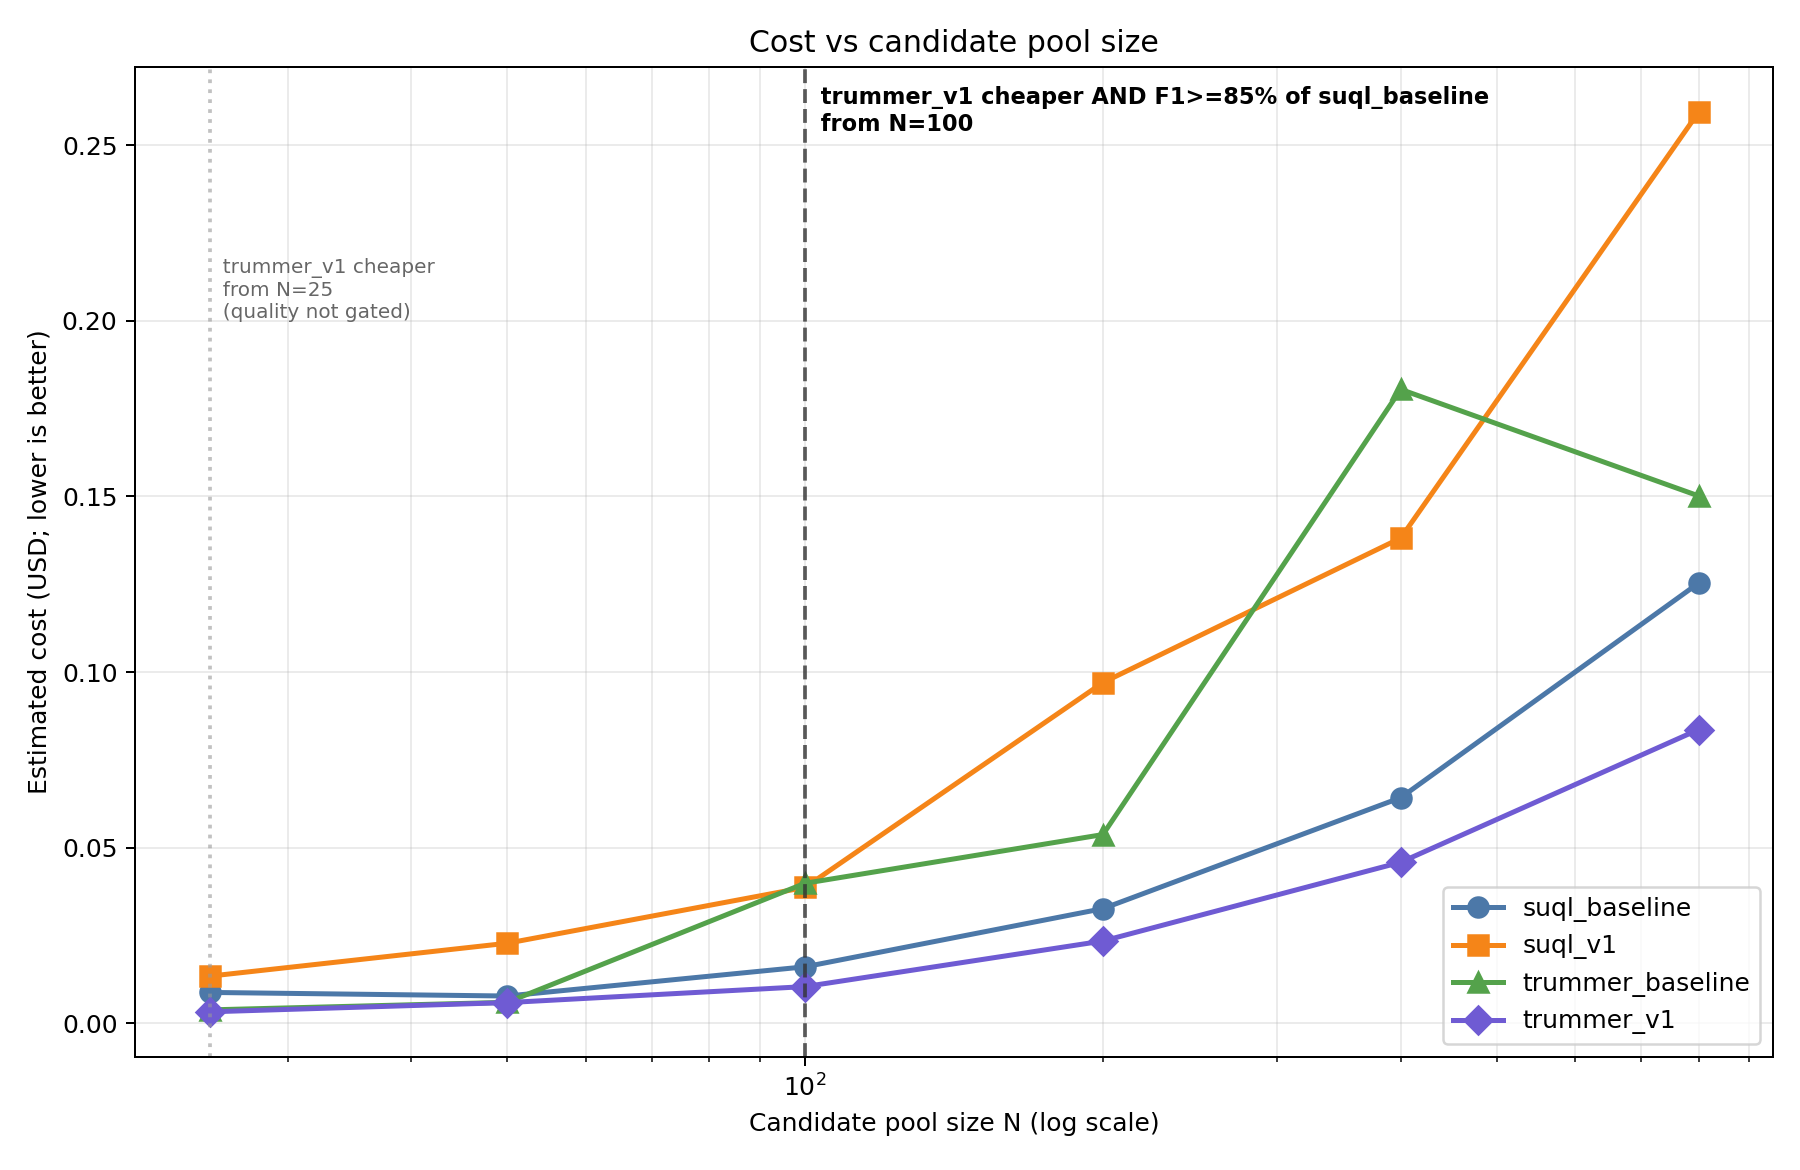
\includegraphics[width=0.85\textwidth]{figs/amazon/01_cost_vs_n.png}
\caption{Estimated \$-cost vs.\ candidate pool size $n$ (log scale),
all four methods.}
\label{fig:amzscale-cost}
\end{figure}

Figure~\ref{fig:amzscale-cost} sweeps pool size on a log axis; because
the underlying cost model is linear in $n$ plus a fixed calibration
term (Proposition~\ref{prop:crossover}), the near-flat-then-rising
shape here is the expected signature of a linear function viewed
against $\log n$, not evidence of super-linear growth. The annotated
threshold marks where Trummer~V1 becomes cheaper than SUQL baseline
(from $n{=}25$, quality not yet gated) and where it is both cheaper and
within $85\%$ of SUQL baseline's F1 ($n{=}100$).

\begin{figure}[h]
\centering
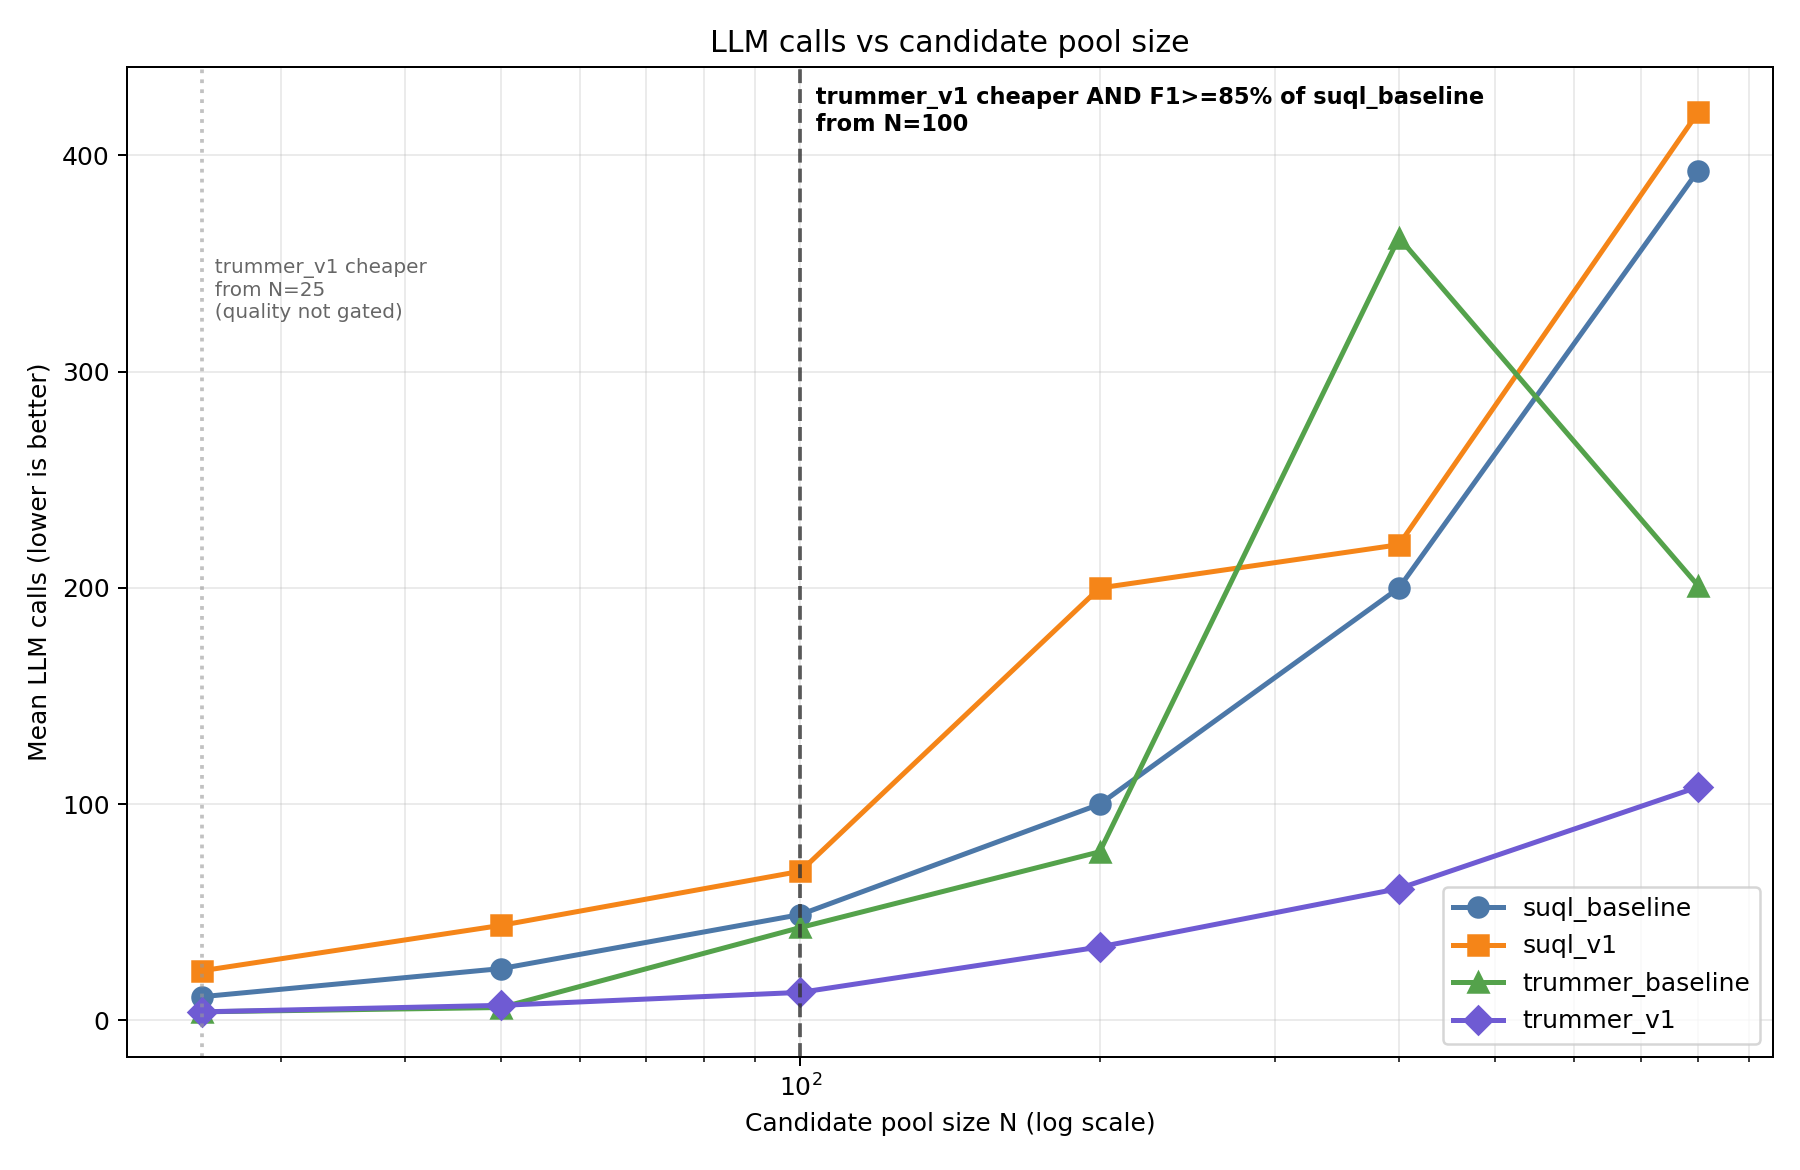
\includegraphics[width=0.85\textwidth]{figs/amazon/02_calls_vs_n.png}
\caption{Mean LLM calls vs.\ candidate pool size $n$ (log scale).}
\label{fig:amzscale-calls}
\end{figure}

Figure~\ref{fig:amzscale-calls} isolates raw call count from \$-cost.
Trummer~V1 (purple) is the lowest line at every $n$ tested; Trummer
baseline (green) is visibly the noisiest -- consistent with its
adaptive block-pairing retrying and re-partitioning depending on
parse success (Section~\ref{sec:trummer-baseline}), unlike the other
three methods' comparatively smooth, near-linear growth.

\begin{figure}[h]
\centering
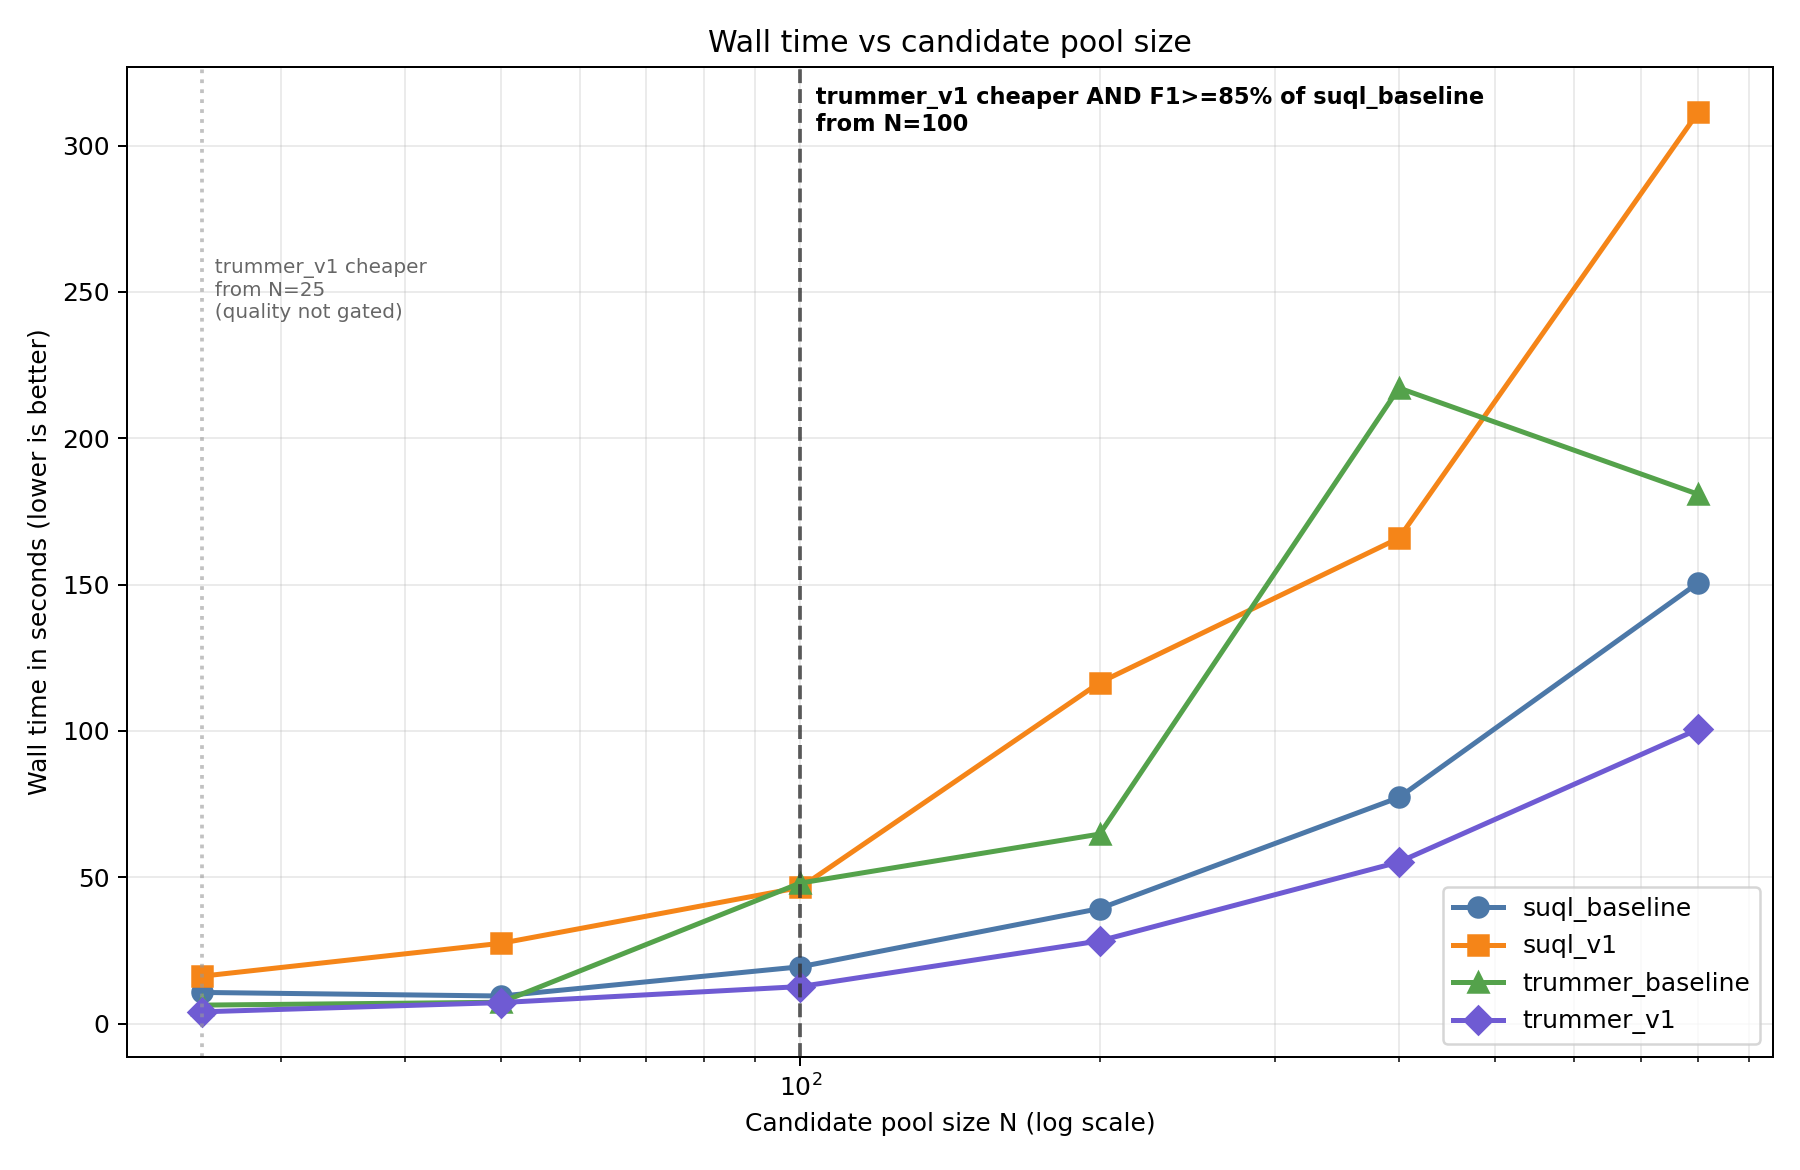
\includegraphics[width=0.85\textwidth]{figs/amazon/03_time_vs_n.png}
\caption{Mean wall time (s) vs.\ candidate pool size $n$ (log scale).}
\label{fig:amzscale-time}
\end{figure}

Figure~\ref{fig:amzscale-time} shows SUQL~V1 (orange) crossing above
even the noisy Trummer baseline by roughly $n{=}150$ and finishing as
the slowest method at $n{=}300$ -- the same qualitative story as the
IMDb result, now shown continuously across a wide range of pool sizes
rather than at one fixed $n$.

\begin{figure}[h]
\centering
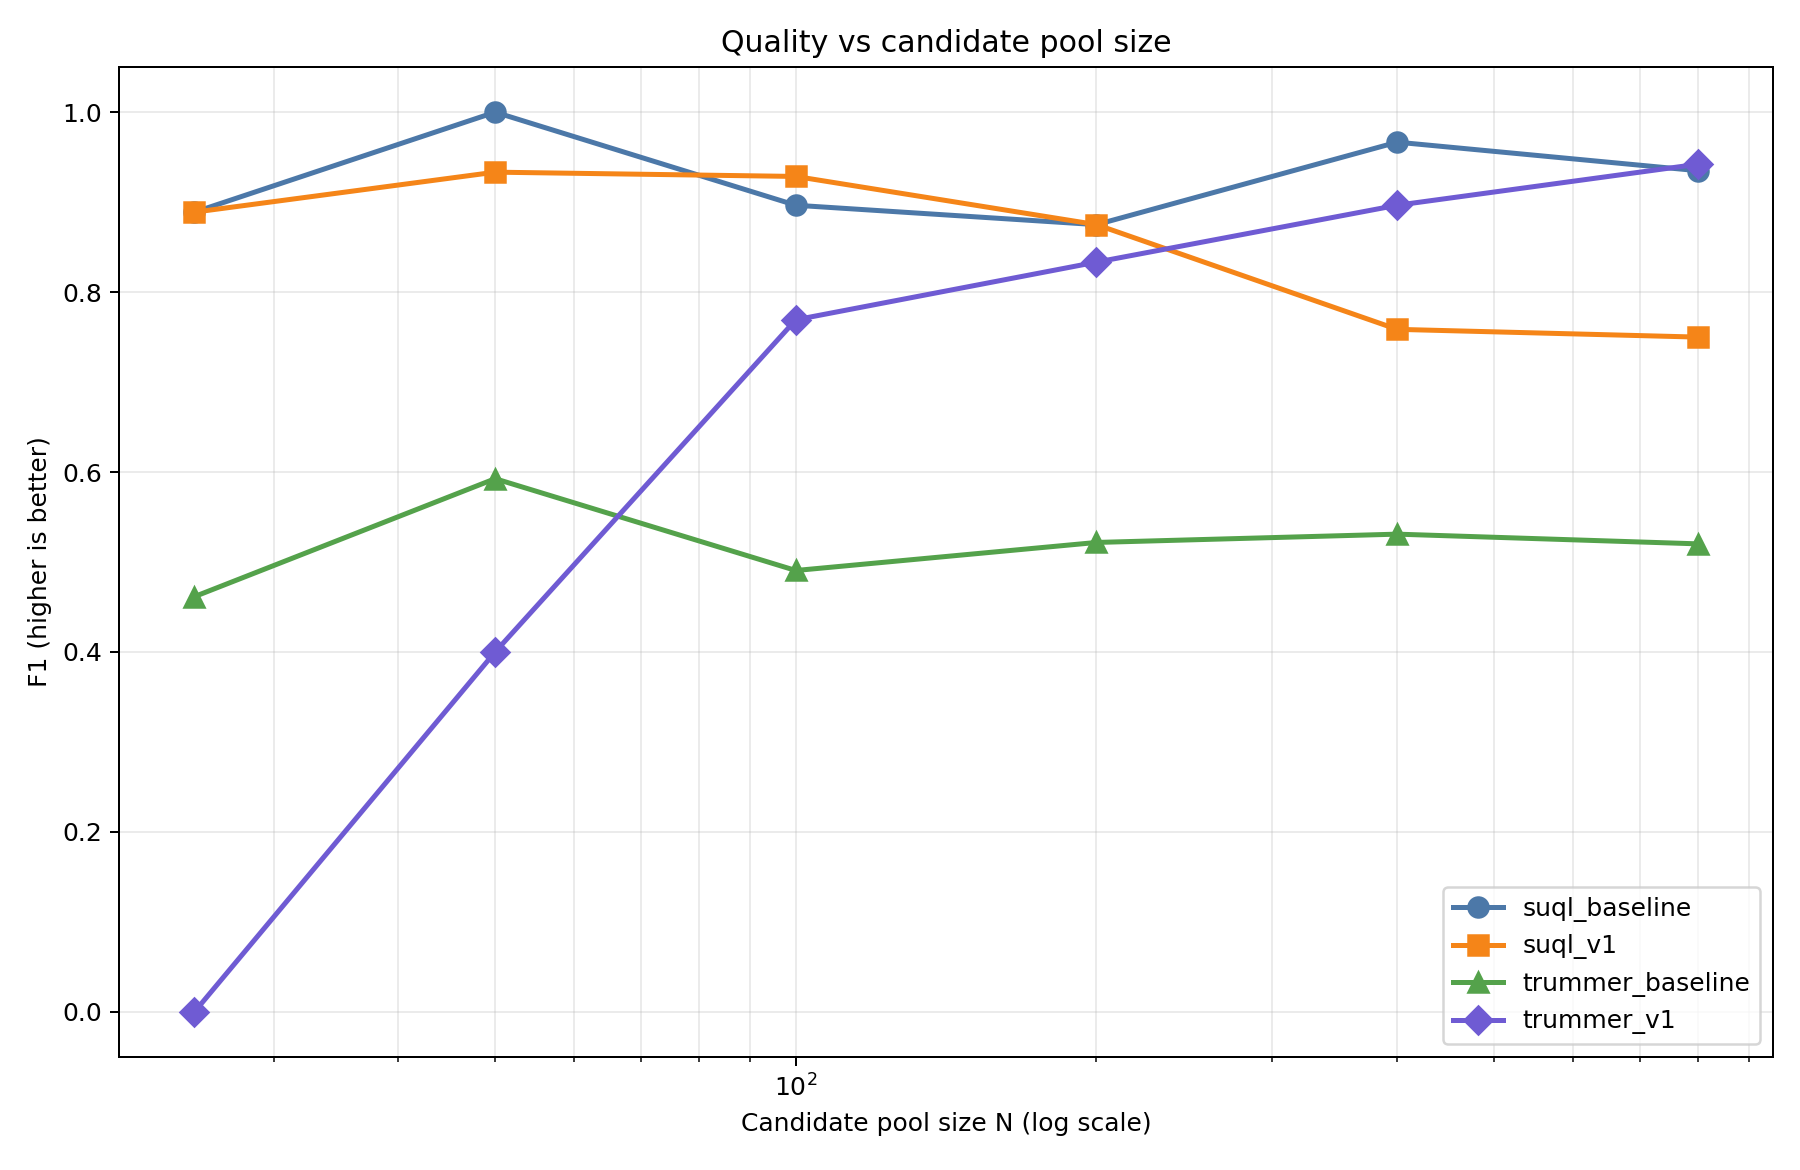
\includegraphics[width=0.85\textwidth]{figs/amazon/04_f1_vs_n.png}
\caption{F1 vs.\ candidate pool size $n$ (log scale).}
\label{fig:amzscale-f1}
\end{figure}

Figure~\ref{fig:amzscale-f1} is the least monotonic of the four: every
method's F1 line bends up and down across the sweep rather than
trending cleanly, and Trummer~V1 (purple) starts at F1 $=0$ for the
smallest pool tested before climbing above every other method by
$n{\gtrsim}150$. This non-monotonicity is discussed below -- it
reflects the escalation rate $\pi$ not being perfectly stable across
differently-sized synthetic pools, and, at the smallest $n$, the
calibration set itself being too small relative to $n$ for the
threshold search to produce a usable band at all.

Computing the empirical failure probability
$\Pr[\text{cascade cost}\ge\text{vanilla cost}]$ from every pairwise
comparison at each $n$: \textbf{on LLM calls, the cascade lost
\emph{zero} times, at every $n$ from $100$ to $300$, in both
regimes} -- including the adversarial one, meaning the measured margin
$\Delta$ beat even a calibration cost that never amortizes away. On
wall time, one small ($0.66\%$) failure rate appears at $n{=}100$,
vanishing by $n{=}125$, consistent with ordinary system-timing jitter.
One honest caveat: \texttt{expensive\_calls} had \emph{zero}
within-$n$ variance here (deterministic cheap-stage decoding), so this
confirms Proposition~\ref{prop:crossover}'s conclusion cleanly without
directly exercising Proposition~\ref{prop:hoeffding}'s Binomial-concentration
mechanism -- a follow-up with a sampling-temperature cheap stage or
freshly-resampled pools per repetition would be needed for that.

Quality is less clean across this sweep: Trummer~V1 loses F1 to the
lean vanilla reference at $2$ of $6$ pool sizes in the dense run and
$4$ of $6$ in calibfrac, tracking a \texttt{calibration\_agreement}
that misses its $0.9$ target at every single point tested ($0.27$--$0.89$).
This reinforces, independently of \S\ref{sec:imdb-vs-amazon-fashion}'s
ten-question comparison, that Trummer~V1's point-estimate calibration
(\S\ref{sec:trummer-v1}) is the more likely source of cross-domain
quality variability than the cascade architecture itself.

\subsection{Qwen vs.\ Gemma on Amazon}
\label{sec:amazon-model-comparison-2}

A Qwen cheap/expensive pair was evaluated on the same Amazon workload,
in a five-question-averaged suite. Table~\ref{tab:qwen-vs-gemma}
compares it against the Amazon Fashion \texttt{10q} Gemma run of
\S\ref{sec:imdb-vs-amazon-fashion} -- a better-matched reference than
the single pool-size point used in an earlier revision, though the
suite sizes still differ (five questions vs.\ ten).

\begin{figure}[h]
\centering

\includegraphics[width=0.85\textwidth]{figs/qwen_amazon/01_quality.png}
\caption{Qwen, Amazon five-question suite: precision, recall, F1
(error bars: std.\ dev.\ across repetitions).}
\label{fig:qwen-quality}
\end{figure}

Figure~\ref{fig:qwen-quality} shows the same precision/recall imbalance
for Trummer baseline under Qwen as under Gemma
(Figure~\ref{fig:amzf-quality}): precision collapses to $0.360$ against
recall $0.907$. SUQL baseline, SUQL~V1, and Trummer~V1 all cluster in a
narrow F1 band ($0.863$--$0.878$), with error bars overlapping
substantially -- the three are not clearly separable on quality alone
under this suite's repetition count.

\begin{figure}[h]
\centering

\includegraphics[width=0.85\textwidth]{figs/qwen_amazon/02_time.png}
\caption{Qwen, Amazon five-question suite: mean wall time, cheap vs.\
expensive stage.}
\label{fig:qwen-time}
\end{figure}

Figure~\ref{fig:qwen-time} again puts SUQL~V1 tallest ($48.3$s,
$77\%$ cheap-stage) and Trummer~V1 shortest ($17.4$s), the same
qualitative ranking as both Gemma runs above, now under a different
model family entirely.

\begin{figure}[h]
\centering

\includegraphics[width=0.85\textwidth]{figs/qwen_amazon/03_calls.png}
\caption{Qwen, Amazon five-question suite: mean LLM calls, cheap vs.\
expensive stage.}
\label{fig:qwen-calls}
\end{figure}

Figure~\ref{fig:qwen-calls} shows SUQL~V1 using \emph{more} total calls
than SUQL baseline ($75.0$ vs.\ $48.6$), matching its Amazon-Fashion
behavior under Gemma (Figure~\ref{fig:amzf-calls}) rather than its
IMDb behavior -- further evidence that the IMDb result was closer to a
best case for SUQL~V1 than a typical one.

\begin{figure}[h]
\centering

\includegraphics[width=0.85\textwidth]{figs/qwen_amazon/04_best_solution.png}
\caption{Qwen, Amazon five-question suite: recall vs.\ wall time,
harness best-solution annotation is Trummer~V1.}
\label{fig:qwen-best}
\end{figure}

Figure~\ref{fig:qwen-best} places all three of SUQL baseline, Trummer
baseline, and Trummer~V1 at broadly similar recall, with SUQL~V1 alone
pulled far to the right on time -- the same isolated-outlier pattern
seen in both Gemma figures (Figures~\ref{fig:imdb-best},
\ref{fig:amzf-best}).

\begin{figure}[h]
\centering

\includegraphics[width=0.85\textwidth]{figs/qwen_amazon/05_cost_by_approach.png}
\caption{Qwen, Amazon five-question suite: estimated \$-cost per
question.}
\label{fig:qwen-cost}
\end{figure}

Figure~\ref{fig:qwen-cost} shows SUQL~V1 as the most expensive method
(\$0.0403) and Trummer~V1 the cheapest (\$0.0145). The per-call
annotations are the basis of the cross-model \$-cost puzzle resolved
below: SUQL~V1's cheap-call cost here (\$0.00062) is identical to its
Gemma/Amazon-Fashion counterpart to five significant figures.

\begin{figure}[h]
\centering

\includegraphics[width=0.85\textwidth]{figs/qwen_amazon/06_cost_vs_f1.png}
\caption{Qwen, Amazon five-question suite: cost--F1 Pareto frontier.}
\label{fig:qwen-pareto}
\end{figure}

Figure~\ref{fig:qwen-pareto} shows the same two-point Pareto frontier
shape as the Gemma/Amazon-Fashion result (Figure~\ref{fig:amzf-pareto}):
Trummer~V1 (\$0.0145, F1 $0.865$) and SUQL baseline (\$0.0175, F1
$0.878$) are both non-dominated, while SUQL~V1 and Trummer baseline are
each dominated on both axes at once.

\begin{table}[h]
\centering\small
\begin{tabular}{lrr}
\toprule
vs.\ SUQL baseline & Qwen (5q) & Gemma (Amazon Fashion, 10q) \\
\midrule
Trummer~V1 $\Delta$F1    & $-1.5\%$  & $-4.3\%$ \\
Trummer~V1 $\Delta$calls & $-80.7\%$ & $-73.6\%$ \\
SUQL~V1 $\Delta$F1       & $-1.7\%$  & $-7.1\%$ \\
SUQL~V1 $\Delta$calls    & $+54.3\%$ & $+59.1\%$ \\
\bottomrule
\end{tabular}
\caption{Both model families now cover all four methods on Amazon data.}
\label{tab:qwen-vs-gemma}
\end{table}

The two model families now agree on \emph{direction} for every
comparison in the table, which they did not in an earlier revision of
this report (that revision's Gemma reference point showed a small
\emph{positive} F1 delta for Trummer~V1, based on one pool-size
measurement rather than a ten-question average; the properly-matched
comparison here shows a small \emph{negative} delta, consistent with
Qwen -- we flag this as a correction rather than silently updating it).
\textbf{Both model families show Trummer~V1 trading a small, consistent
amount of F1 ($1.5$--$4.3\%$) for a large, consistent reduction in
calls ($74$--$81\%$), and both show SUQL~V1 strictly dominated by its
own baseline on Amazon data} -- worse on calls, time, and F1 at once.
This is the clearest cross-model evidence in either report that the
cost mechanism (structured pushdown, batching) is architecture-level
and portable, while SUQL~V1's specific unbatched design is the outlier
that does not travel well.

A puzzle from an earlier revision of this report is now resolved rather
than merely flagged: SUQL~V1's reported per-call \$-cost is nearly
identical across the Qwen and Gemma Amazon runs (cheap $\$0.00062$ in
both; expensive $\$0.00036$ vs.\ $\$0.00033$). Section~\ref{sec:imdb-plots}'s
IMDb \$-cost breakdown confirms the mechanism: this harness's \$-cost
estimate is simply recorded model service \emph{time} multiplied by a
flat \$3.00/accelerator-hour rate, with no per-model price
differentiation, so two runs with similar per-call \emph{latency} will
show similar \$-costs regardless of which underlying model produced
that latency. The near-identical figures are therefore evidence that
SUQL~V1's cheap-stage latency happened to be similar under both model
labels, not evidence that the two runs shared an underlying model.

\paragraph{Remaining scope.} Neither run reports specific model
parameter counts (only ``cheap''/``expensive'' role labels), so the
exact ratio $P_c/P_e$ cannot yet be stated for the Qwen pair the way
Table~\ref{tab:theory-constants} does for Gemma. Both model families
now cover all four methods on Amazon data, closing the coverage gap
noted in an earlier revision of this report.

\section{Discussion}

\textbf{Structured selectivity still dominates wall time.} Across all
four variants, and now confirmed over ten diverse questions rather than
one, the wall-clock gap between the SUQL and Trummer families tracks how
many rows survive structured pushdown before any semantic operator runs;
every question in this suite fixes the structured candidate count at
$40$ out of $100$, so the ranking we report is specific to this
$40\%$-selectivity regime and should be re-measured at other
selectivities before being treated as universal.

\textbf{The \answerfn{} yield rate remains a useful label-free
diagnostic}, unchanged from earlier analysis: very high acceptance
of structurally-filtered rows indicates an under-specified predicate,
very low acceptance suggests over-constraint or a vocabulary mismatch,
and both are visible without any gold labels at all.

\textbf{\texttt{LIMIT} without early termination} remains an
unaddressed, self-contained optimization opportunity: none of the four
implementations currently stop evaluating the semantic operator early
once a \texttt{LIMIT k} clause's target has been met.

\textbf{Threats to validity, updated.} The \texttt{10q} suite directly
answers the single-query threat flagged previously, but a new,
narrower one appears in its place: every question in this suite shares
the same $100/40/12$ structural shape by design, so the reported
numbers characterize behavior at one fixed selectivity and one fixed
gold-set size, not a selectivity sweep. The repository's \texttt{1q},
\texttt{3q}, and \texttt{5q} suites, and the previously sketched
20-query ablation, remain the natural next steps toward a full
selectivity-by-difficulty grid (Chapter~\ref{chap:conclusion}).

\chapter{Conclusion and Future Work}
\label{chap:conclusion}

\section{Summary}

This report set out to answer a concrete systems question: given a
heterogeneous data pool mixing structured columns and free-text reviews,
how should a query engine execute a natural-language question that
mixes a structured predicate with a semantic one, while controlling both
LLM invocation cost and wall-clock latency? We benchmarked two baseline
strategies -- row-wise predicate pushdown (SUQL~\cite{suql}) and an
adaptive, join-based batched strategy in the style of Trummer -- and
found them to occupy different points of the cost/quality trade-off
space, now validated over ten held-out, genre-diverse questions rather
than one (Chapter~\ref{chap:experiments}). We introduced a two-level
cascade, applicable on top of either baseline, in which a cheap
first-stage scorer resolves the majority of units of work immediately
and escalates only genuinely ambiguous units to an expensive verification
step. The cascaded batched design, Trummer~V1, dominated on every axis
we measured: best F1 ($0.757$), best precision ($0.810$), the highest
\emph{floor} across the ten questions ($0.500$, versus $0.267$ or lower
for every other method), and by far the lowest cost ($10.0$ calls,
$35.05$s per question) -- at a small ($\approx 7\%$ relative) recall cost
compared to the cascaded row-wise design. New in this revision, we also
proved -- rather than only observed -- \emph{why}: a calibrated cascade's
expected and (with high, exponentially-growing probability) realized
cost is lower than an all-expensive baseline's once the candidate pool
is large enough, provided the cheap stage's batching factor and
calibrated escalation rate satisfy an explicit margin condition
(Section~\ref{sec:theory-cost}). Plugging in the measured system
constants shows SUQL~V1 fails that margin condition on both calls and
time (explaining its wall-time regression analytically, not just
empirically), while Trummer~V1 satisfies it comfortably on both.

\section{Engineering Lessons}

Beyond the headline numbers, four lessons from this project generalize
beyond this specific workload:
\begin{enumerate}
  \item \textbf{Predicate pushdown is the dominant cost lever} --
        confirmed, not just asserted, by the fact that the one method in
        the Trummer family that adds it (Trummer~V1) is also the only
        one that is both fast \emph{and} accurate.
  \item \textbf{Batching the cheap stage is not an optimization detail
        -- it determines whether cascading can win on cost or time at
        all.} Section~\ref{sec:theory-cost}'s worked instantiation shows
        this precisely: SUQL~V1's unbatched ($B=1$) cheap stage cannot
        satisfy the theorem's margin condition under its current
        per-call latency, while Trummer~V1's batched ($B=8$) cheap stage
        satisfies it with room to spare.
  \item \textbf{Calibration conventions are a real source of bugs.} The
        $\alpha$-as-confidence-level vs.\ $\alpha$-as-tail-probability
        pitfall of Section~\ref{sec:quantile-pitfall} produced two
        individually defensible formulas, only one of which matched the
        calling code's own convention; only a regression test against a
        synthetic confusion matrix with a known closed-form answer
        caught it.
  \item \textbf{A single hand-verified query is not enough to trust a
        cost/quality comparison.} Moving from one query to the
        \texttt{10q} suite changed the story in a material way: it
        surfaced Trummer~V1's floor-robustness (invisible in a
        single-query comparison, since there is no floor to speak of
        with $n=1$) and it exposed a genuinely hard question (Q3,
        romance chemistry) on which two of the four methods nearly
        collapse -- exactly the kind of finding a broader benchmark
        suite is for.
\end{enumerate}

\section{Current Implementation Status}

At the time of writing, all four methods -- SUQL baseline/V1, Trummer
baseline/V1 -- are implemented, documented, and benchmarked end to end
in the public repository
(\url{https://github.com/AnnaRemi/ENSIMAG-AI-M2-final-project}, branch
\texttt{agent/consolidate-four-method-benchmarks}), with a shared runner
and evaluator (\texttt{benchmarks/shared/scripts/}) producing the
\texttt{aggregate.csv}, \texttt{comparison.csv}, and per-question plots
this report draws on. Four benchmark suites of increasing size
(\texttt{1q}, \texttt{3q}, \texttt{5q}, \texttt{10q}) are available and
runnable locally (against a local Ollama instance) or on the lab's
shared Aker cluster.

\section{Future Work}

\subsection{Batch SUQL~V1's cheap stage}
\label{sec:future-suql-v1}
Section~\ref{sec:theory-cost}'s analysis makes this the single most
consequential remaining change: SUQL~V1's cheap stage currently scores
one row per call ($B=1$), and its measured per-row latency already
exceeds the expensive stage's own per-call latency, which
Proposition~\ref{prop:crossover} shows makes a wall-time win
\emph{structurally impossible} regardless of calibration quality or
pool size. Batching the cheap probe (scoring several rows' log-odds in
one completion, the same lever that already makes Trummer~V1's cheap
stage effective) is predicted, by the same analysis, to be the change
most likely to convert SUQL~V1 from a quality-only cascade into one that
also wins on cost and time.

\subsection{Port Beta-posterior calibration to Trummer~V1}
As flagged in Section~\ref{sec:trummer-v1}, Trummer~V1's threshold is
currently learned by a point-estimate agreement search rather than the
Beta-posterior credible-bound procedure used by SUQL~V1
(Section~\ref{sec:beta-posterior}). The two are not equally rigorous:
only the Beta-posterior version currently carries an explicit,
finite-sample confidence-level guarantee. Unifying both cascades on the
same calibration procedure would let Trummer~V1 -- already the strongest
variant on every other axis -- also carry that guarantee.

\subsection{Amortize the calibration budget across repeated queries}
Both cascades currently re-run their calibration procedure fresh for
every question ($K_{\mathrm{calls}}=20$ row-wise calls for SUQL~V1,
$1$ batched call for Trummer~V1, per Table~\ref{tab:theory-constants}).
In a deployment that re-asks a stable set of semantic predicates
repeatedly (\eg a fixed catalogue of recommendation filters), this cost
is payable once and amortized over every future invocation of the same
predicate, pushing the crossover point $n^\ast$ of
Proposition~\ref{prop:crossover} even lower than the already-small value
computed for Trummer~V1 in Section~\ref{sec:worked-instantiation}.

\subsection{The KV-cache-aware execution ladder}
\label{sec:future-kv-cache}
Stretto's second contribution -- \emph{Expected Attention Press}, a
cache-aware execution ladder that reuses attention key/value state
across cascade stages -- remains deliberately deferred. It requires
direct access to the serving engine's attention state (\eg via
\texttt{vllm}), which an Ollama-served backend does not expose; adopting
it is future work contingent on a backend migration, and remains the
single largest piece of remaining architectural work identified by this
project.

\subsection{Extending the selectivity/difficulty grid}
\label{sec:future-ablation}
The \texttt{10q} suite fixes structural selectivity at $40\%$
(Chapter~\ref{chap:experiments}); the repository's smaller \texttt{1q},
\texttt{3q}, and \texttt{5q} suites, and a still-larger suite beyond
\texttt{10q}, are the natural next steps toward a full grid crossing
structural selectivity with semantic-predicate difficulty, which would
let the cost/quality trade-offs of this report be stated as trends
across that grid rather than at one fixed selectivity.

\subsection{Early termination for \texttt{LIMIT} queries}
As discussed in Chapter~\ref{chap:experiments}, wiring early stopping
into the cascade's main accept loop once $|\mathit{Accept}| \ge k$ for a
\texttt{LIMIT k} query remains a small, self-contained, and still
unimplemented optimization.

\appendix
\chapter{Prompts and Reproduction Reference}
\label{chap:appendix}

\section{Complete Prompt Reference}

For convenience, this section collects every prompt referenced in the
body of the report in one place. All are transcribed verbatim (module
docstrings/comments removed) from
\url{https://github.com/AnnaRemi/ENSIMAG-AI-M2-final-project/tree/agent/consolidate-four-method-benchmarks}.

\begin{lstlisting}[style=prompt, caption={SUQL baseline \answerfn{} system prompt (\texttt{project SUQL/baseline/suql\_engine.py}).}]
You are a recall-first semantic filter for movie reviews.

Decide whether the review provides evidence that the movie
satisfies the question.

Recall is the primary objective, but do not accept every
review:
- Answer YES when there is any concrete review-specific
  evidence: direct wording, a synonym/paraphrase, a described
  example, or a reasonable implication.
- Give borderline evidence the benefit of the doubt when it
  specifically bears on the condition. The evidence need not
  use the question's exact words.
- This is evidence retrieval, not sentiment scoring: an
  explicit mention still counts when it is negated, qualified,
  quoted, or used critically.
- Answer NO when there is no review-specific support, the
  connection is only the movie's genre/topic, the text is
  generic praise or criticism, or the review never discusses
  the condition itself.
- Do not infer evidence merely because the condition is not
  contradicted.

Return exactly YES or NO. Do not include reasoning,
punctuation, or extra text.
\end{lstlisting}

\begin{lstlisting}[style=prompt, caption={SUQL semantic-parser system prompt (\texttt{project SUQL/baseline/suql\_engine.py}, \texttt{PARSER\_SYSTEM}), which compiles the NL question into a SUQL query.}]
You are a SUQL (Structured and Unstructured Query Language)
semantic parser.
SUQL extends SQL with two free-text functions:
  answer(free_text_column, 'question') -> 'Yes'|'No'|short string
  summary(free_text_column)             -> a short prose summary

{TABLE_SCHEMA}

Rules:
1. Use plain SQL WHERE clauses for ALL structured predicates
   (year, runtime, director, genres, title, movie_id).
2. Use answer() ONLY for predicates that require understanding
   the review text.
3. Always apply structured filters BEFORE answer() in the
   WHERE clause (efficiency).
4. The SELECT list must include: movie_id, title, year,
   runtime, director, genres. Add summary(review) AS
   review_summary whenever you use answer() on the review.
5. Use LIKE '%value%' for partial text matches on genres and
   director.
6. For "top N" questions without a numeric ranking field, use
   LIMIT N.
7. Output ONLY the raw SQL query -- no markdown fences, no
   explanation.

{FEW_SHOT_EXAMPLES}
\end{lstlisting}

\begin{lstlisting}[style=prompt, caption={Trummer baseline block-join prompt (\texttt{project Trummer/baseline/trummer\_join/operators.py}, \texttt{create\_prompt}).}]
Find every movie in Collection 1 that has a review in
Collection 2 satisfying this predicate:
{predicate}
Act as a recall-first semantic filter, while requiring
review-specific evidence.
- Answer YES for direct wording, synonyms/paraphrases,
  described examples, or reasonable implications.
- Give borderline evidence the benefit of the doubt when it
  specifically bears on the predicate.
- Count explicit mentions even when negated, qualified,
  quoted, or critical; retrieve evidence rather than score
  sentiment.
- Answer NO when support is absent, generic, based only on
  genre/topic, or never discusses the predicate itself.
- Lack of contradiction alone is not evidence.
Collection 1 contains structured movie rows. Collection 2
contains review chunks.
A review belongs to a movie only when tconst is exactly
equal to movie_id.
Return one decision per line as: movie_id: YES or
movie_id: NO.
Do not include confidence, evidence, explanations, or prose.
Copy each movie_id exactly from Collection 1.
Do not add prose, JSON, markdown, or a completion marker.

Collection 1:
{block_1_rows}

Collection 2:
{block_2_rows}

Decisions:
\end{lstlisting}

\begin{lstlisting}[style=prompt, caption={SUQL~V1 cheap Stage~1 single-token scoring prompt (\texttt{project SUQL/v1/scorer.py}).}]
Act as a high-recall first-pass semantic filter. Decide
whether this review contains review-specific evidence for a
Yes answer. Count direct wording, synonyms, described
examples, and reasonable implications as evidence. Give
borderline but condition-specific evidence the benefit of
the doubt. Do not discard an explicit mention because it is
negated, qualified, quoted, or critical: this is evidence
retrieval, not sentiment scoring. Do not count genre/topic
alone, generic praise or criticism, or mere lack of
contradiction as evidence.
Return exactly one token: 1 for Yes, 0 for No.

Question: {question}
Review: {review[:1800]}

Answer:
\end{lstlisting}

\begin{lstlisting}[style=prompt, caption={SUQL~V1 expensive Stage~2 verification prompt (\texttt{project SUQL/v1/cascade\_filter.py}, \texttt{ANSWER\_SYSTEM}).}]
You are the final recall-first semantic filter for movie
reviews.

Decide whether the review provides evidence that the movie
satisfies the question.

Recall is the primary objective, but do not accept every
review:
- Answer YES for any concrete review-specific support,
  including direct wording, synonyms, described examples, and
  reasonable implications.
- Give borderline evidence the benefit of the doubt when it
  specifically bears on the condition; exact wording is
  unnecessary.
- This is evidence retrieval, not sentiment scoring: an
  explicit mention still counts when it is negated, qualified,
  quoted, or used critically.
- Answer NO when support is absent, merely generic, based only
  on genre/topic, or never discusses the condition itself.
  Lack of contradiction alone is not evidence.

Return exactly YES or NO. Do not include reasoning,
punctuation, or extra text.
\end{lstlisting}

\begin{lstlisting}[style=prompt, caption={Trummer~V1 cheap Stage~1 batched prompt (\texttt{project Trummer/v1/trummer\_join/cascade.py}, \texttt{\_cheap\_batch\_prompt}).}]
Classify every explicit candidate pair below.
Predicate: {predicate}
{CHEAP_EVIDENCE_INSTRUCTIONS}
Return one line per candidate as CANDIDATE_ID: YES, NO, or
UNCERTAIN.
Do not include confidence, evidence, explanations, or prose.
Return every candidate exactly once and do not explain.

CANDIDATE_{n}:
Movie: {movie_text}
Review: {review_text}
...

Decisions:
\end{lstlisting}

\begin{lstlisting}[style=prompt, caption={Trummer~V1 expensive Stage~2 batched verification prompt (\texttt{cascade.py}, \texttt{\_expensive\_batch\_prompt}).}]
Evaluate the explicit candidate pairs below.
Predicate: {predicate}
{EXPENSIVE_EVIDENCE_INSTRUCTIONS}
Return one line per candidate as PAIR_ID: YES or PAIR_ID: NO.
Do not include confidence, evidence, explanations, or prose.
Return every candidate exactly once. Do not add prose, JSON,
or markdown.

PAIR_{n}:
Movie: {movie_text}
Review: {review_text}
...

Decisions:
\end{lstlisting}

\section{Calibration Reference Values}
\label{sec:appendix-calibration}

Table~\ref{tab:appendix-thresholds} lists the calibrated cheap-stage
accept/reject log-odds thresholds actually stored in
\texttt{project SUQL/v1/thresholds.json} for a representative sample of
predicates from earlier (pre-\texttt{10q}) calibration runs; the
\texttt{10q} benchmark of Chapter~\ref{chap:experiments} recalibrates
fresh per question rather than reusing this file, but the values
illustrate the typical magnitude of the calibrated band.

\begin{table}[h]
\centering\small
\begin{tabular}{p{9.5cm}rr}
\toprule
Predicate (abbreviated) & Accept $\tau_+$ & Reject $\tau_-$ \\
\midrule
Funny, humorous, witty, or entertaining? & $1.0$ & $-1.0$ \\
Praise acting/performances/cast/characters? & $1.0$ & $-1.0$ \\
Suspense, tension, scares, fear, creepy atmosphere? & $1.0$ & $-1.0$ \\
Praise chemistry, romance, love story, relationships? & $1.0$ & $-1.0$ \\
Exciting, thrilling, intense, action-packed? & $1.0$ & $-1.0$ \\
\bottomrule
\end{tabular}
\caption{Sample calibrated thresholds, \texttt{project SUQL/v1/thresholds.json}.
The symmetric $\pm 1.0$ band corresponds to routing everything with
cheap-stage probability outside roughly $[0.27, 0.73]$ directly, and
escalating the rest.}
\label{tab:appendix-thresholds}
\end{table}

\section{Reproduction: Running the Benchmarks Locally}
\label{sec:appendix-cli}

The repository's runner supports all four methods and all four suite
sizes out of the box; the commands below are the actual entry points
(not a hypothetical interface), taken from the repository's top-level
and \texttt{benchmarks/} README files.

\begin{lstlisting}[style=prompt, caption={Cloning and running the smoke-test suite locally against Ollama.}]
git clone git@github.com:AnnaRemi/ENSIMAG-AI-M2-final-project.git
cd ENSIMAG-AI-M2-final-project
bash benchmarks/1q/run_local.sh --pull-models
\end{lstlisting}

\begin{lstlisting}[style=prompt, caption={Running the full 10-question, 10-repetition suite on the lab's Aker cluster (the exact configuration used to produce Chapter~\ref{chap:experiments}'s tables).}]
bash benchmarks/run_aker.sh \
  --suite 10q \
  --repetitions 10 \
  --methods "suql_baseline suql_v1 trummer_baseline trummer_v1" \
  --cheap-model gemma4:e2b \
  --expensive-model gemma4:26b \
  --pull-models
\end{lstlisting}

Both entry points create a \texttt{.venv}, install the shared Python
dependencies, pull the configured models, verify the local Ollama API,
and run all four implementations end to end, writing
\texttt{aggregate.csv}, \texttt{comparison.csv}, and the four aggregate
plots (quality, time, call-count, and a speedup-vs-call-reduction
scatter, plus per-question versions of the same four plots) to
\texttt{benchmarks/<suite>/outputs/<run-name>/}. Raw model responses and
per-repetition intermediate artifacts are deleted after successful
evaluation by default (pass \texttt{--keep-run-artifacts} to
\texttt{shared/scripts/run\_all.py} directly to retain them for
debugging).

%=========================================================


%=========================================================
\backmatter

\bibliographystyle{plain} % plain-fr si rapport en fran\c{c}ais
\bibliography{bibfile}

%\cleardoublepage % Goes to an odd page
%\pagestyle{empty} % no page number
%~\newpage % goes to a new even page

\end{document}
